\documentclass{article}
\usepackage{graphicx}
\usepackage{amsfonts}
\usepackage{enumitem}
\usepackage{pmboxdraw}
\usepackage{nicematrix}
\usepackage[T1]{fontenc}
\usepackage{lmodern}
\usepackage{microtype}
\usepackage{multicol}
\usepackage[dvipsnames]{xcolor}
\usepackage{eso-pic}
\usepackage{booktabs}
\usepackage{menukeys}
\renewmenumacro{\menu}{angularmenus}
\renewmenumacro{\keys}{shadowedangularkeys}
\renewmenumacro{\directory}{pathswithfolder}
\usepackage{ccicons}
\usepackage{tikz}
\usepackage{pgfplots}
\usepgfplotslibrary{polar}
\pgfplotsset{compat=1.18}
\definecolor{linkcolor}{RGB}{40, 70, 120}
\usepackage{caption}
\usepackage[top=1in, bottom=1in, left=1in, right=1in]{geometry}
\usepackage{colortbl}
\newtheorem{theorem}{Theorem}
\usepackage{tcolorbox}
\usepackage{float}
\tcbuselibrary{listings}
\usetikzlibrary{decorations.pathreplacing, calligraphy}
\usetikzlibrary{shapes.geometric} 
\tcbuselibrary{skins, breakable}
\usepackage{bm}
\usepackage{mdframed}
\usepackage{tocloft}
\usepackage{minted}
\usepackage{titlesec}
\setminted[bash]{
    style=tango,
    breaklines=true,
    frame=single,
    framesep=0mm,
    rulecolor=\color{gray},
    bgcolor=black!5,
    fontsize=\small,
    numbers=left,
    numbersep=5pt
}
\definecolor{codebg}{gray}{0.93}
\newcommand{\code}[1]{\colorbox{codebg}{\texttt{#1}}}
\titleformat{\section}
  {\Large\bfseries\scshape}{\thesection.}{0.5em}{}[\titlerule]
\titleformat{\subsection}
  {\large\bfseries\scshape}{\thesubsection.}{0.5em}{}
  [\vspace{1pt}\hspace{2em}\rule{\dimexpr\textwidth-2em\relax}{0.4pt}]

\titleformat{\subsubsection}
  {\normalsize\bfseries\scshape}{\thesubsubsection.}{0.5em}{}
  [\vspace{1pt}\hspace{4em}\rule{\dimexpr\textwidth-4em\relax}{0.4pt}]
\renewcommand{\cftsecleader}{\cftdotfill{\cftdotsep}} 
\usetikzlibrary{calc}
\newmdenv[linewidth=2pt, linecolor=black!60, topline=false, bottomline=false, rightline=false, backgroundcolor=teal!5!white, frametitle={\small\textbf{Definition}},
frametitlefont=\small\bfseries]{definition}
\newcounter{exercise}
\newcommand{\exercise}{%
  \stepcounter{exercise}%
  \noindent\textbf{Exercise \theexercise.}\quad
}
\newtcolorbox{callout}[1]{
  enhanced,
  colback=calloutbg,
  colframe=calloutborder,
  fonttitle=\bfseries\normalsize,
  title={#1},
  boxrule=0.6pt,
  arc=2pt,
  left=10pt, right=10pt, top=6pt, bottom=6pt,
  borderline west={3pt}{0pt}{calloutborder},
}
\definecolor{inkblack}{HTML}{1A1A1A}
\definecolor{stepblue}{HTML}{1E3A5F}
\definecolor{ruleblue}{HTML}{2E6DA4}
\definecolor{calloutbg}{HTML}{F4F7FB}
\definecolor{calloutborder}{HTML}{2E6DA4}
\definecolor{nordBlue}{HTML}{5E81AC}
\definecolor{nordBlueLight}{HTML}{D8E4F0}
\definecolor{moderngreen}{HTML}{2D6A4F}
\definecolor{moderngreenlight}{HTML}{D8F3DC}
% Colors
\definecolor{terminalgray}{HTML}{808080}
\definecolor{terminalgreen}{HTML}{00FF00} 
\definecolor{terminalred}{HTML}{FF0000} 

% Terminal style box
\newtcblisting{linuxterminal}{
    colback=black,
    coltext=white,
    colframe=black,
    arc=0mm,
    width=1\textwidth, % Increased width to fit longer lines
    center,               % Centers the oversized box on the page
    top=3mm,
    bottom=3mm,
    left=2mm,
    right=2mm,
    listing only,
    listing options={
        basicstyle=\ttfamily\small,
        breaklines=true,
        columns=fullflexible,
        keepspaces=true,
        escapeinside={(*}{*)}
    }
}

% Styled components

\newcommand{\gbox}[1]{%
\textcolor{terminalgray}{[}%
\makebox[2.5em] [c]{\textcolor{terminalgreen}{#1}}%
\textcolor{terminalgray}{]}%
}

\newcommand{\rbox}[1]{%
\textcolor{terminalgray}{[}%
\makebox[8.5em][c]{\textcolor{terminalred}{#1}}%
\textcolor{terminalgray}{]}%
}

\newcommand{\graytext}[1]{\textcolor{terminalgray}{#1}}
\newcommand{\errtext}[1]{\textcolor{terminalred}{#1}}
\newcommand{\spc}{\hspace{3.7em}}


\usepackage[colorlinks=true, urlcolor=linkcolor, linkcolor=black]{hyperref}

\begin{document}
 
 \begin{titlepage}

\AddToShipoutPictureBG*{%
  \AtPageLowerLeft{%
    \begin{tikzpicture}[overlay, remember picture]
      
      \draw[line width=2pt, color=black!80, rounded corners=15pt] 
        ($(current page.south west) + (0.5in,0.5in)$) 
        rectangle 
        ($(current page.north east) - (0.5in,0.5in)$);
      
      \draw[line width=0.7pt, color=black!60, rounded corners=12pt] 
        ($(current page.south west) + (0.55in,0.55in)$) 
        rectangle 
        ($(current page.north east) - (0.55in,0.55in)$);
    \end{tikzpicture}%
  }%
}
\begin{center}
\hspace{0pt}\\
\vspace{4cm}
{\Large \textbf{Principal Author}: \textit{\href{https://www.reddit.com/u/Significant-Wrap-589/s/LexVz3vvN0}{u/Significant-Wrap-589}}}\\[5pt]
{\Large \textbf{Co-Author \& Document Designer}: \textit{\href{https://www.reddit.com/u/MurkyUnit3180/s/QuyAn31plr}{u/MurkyUnit3180}}}\\[3cm]
{\scalebox{2}{\Huge\bfseries LINUX}}\\
\vspace{0.8cm}
{\LARGE\bfseries A BRIEF GUIDE TO}\\[10pt]
{\LARGE\bfseries GAMING}\\

\vfill
    {\normalsize\itshape A collaborative guide for the Linux community}\\[4pt]
    {\small Version 1.0 \(\cdot\) May 2026 \(\cdot\) Licensed under \ccbysa~4.0} \\[2pt]
    {\small\textit{This guide is a living document and will be updated over time.}}
\end{center}
\end{titlepage}

\clearpage
\phantomsection
\pdfbookmark{\contentsname}{toc}
\tableofcontents
\vspace{1em} 
\hrule
\clearpage

\section{What is Linux?}

At its most precise, Linux is not an operating system; it is a kernel. The \textit{kernel} is the core program that sits between your hardware and everything else running on your machine. It manages the CPU, memory, storage, and peripheral devices. As the GNU Project puts it:

\begin{mdframed}[linewidth=1.5pt, linecolor=black!50, topline=true, bottomline=true,
  leftline=false, rightline=false, backgroundcolor=black!3]
  \small\itshape
  ``Linux is the kernel: the program in the system that allocates the machine's resources to the other programs that you run. The kernel is an essential part of an operating system, but useless by itself.''\\[4pt]
  \normalfont\small --- \href{https://www.gnu.org/gnu/linux-and-gnu.en.html}{GNU Project, gnu.org}
\end{mdframed}

\noindent What most people call ``Linux'' is more accurately a \textbf{GNU/Linux distribution}, the kernel bundled with system software, a package manager, a desktop environment,
and various tools that make it a complete, usable OS.

According to \href{https://www.kernel.org/linux.html}{kernel.org}, Linux was originally written from scratch by Linus Torvalds as a Unix-like system, targeting POSIX compliance, with support for true multitasking, virtual memory, and shared libraries. It was first developed for 32-bit x86 PCs but today runs on virtually every processor architecture in existence.

\subsection{How a Linux System Is Structured}

A complete Linux system consists of several layers:

\begin{itemize}[leftmargin=1.5em, nosep, label={\tiny\textbullet}]
  \item \textbf{Bootloader}: loads the OS on startup (e.g.\ GRUB)
  \item \textbf{Kernel}: manages hardware, memory, and processes
  \item \textbf{Init system}: bootstraps user space after boot (typically \code{systemd})
  \item \textbf{Shell}: your interface to the system (e.g.\ \code{bash}, \code{zsh})
  \item \textbf{Desktop Environment}: the graphical layer (e.g.\ GNOME, KDE Plasma)
  \item \textbf{Package Manager}: installs and manages software
\end{itemize}

\begin{tcolorbox}[arc=12pt, outer arc=10pt, 
colback=blue!4!white, colframe=blue!40!black, title=\textbf{Kernel $\neq$ OS}]
 If someone hands you ``the Linux kernel'', you cannot use it as a desktop system. You need a full \textit{distribution}, which packages the kernel with everything else. When people say they ``run Linux'', they mean a distribution like Ubuntu, Arch, or Fedora.
\end{tcolorbox}

\subsection{What is a Distribution?}

A \textbf{distribution} (or \textit{distro}) is a complete operating system built around the Linux kernel. Different distros make different choices about which desktop environment, package manager, and software to include. The kernel itself is the same, only what surrounds it differs. Common package managers you will encounter:

\begin{itemize}[leftmargin=1.5em, nosep, label={\tiny\textbullet}]
  \item \code{apt}: Debian, Ubuntu, Pop!\_OS
  \item \code{dnf}: Fedora
  \item \code{pacman}: Arch Linux, Manjaro
\end{itemize}

\noindent To update your system, the command looks like this depending on your distro:

\begin{minted}{bash}
# Debian/Ubuntu
sudo apt update && sudo apt upgrade

# Fedora
sudo dnf upgrade

# Arch
sudo pacman -Syu

\end{minted}

\noindent Keeping your system updated is not optional, it is the foundation of a stable gaming setup. On Linux, drivers, compatibility layers like \textit{Proton}, and core libraries like \textit{glibc} and \textit{Mesa} all ship through the package manager. An outdated system means outdated graphics drivers, which directly translates to lower performance, crashes, or games outright refusing to launch.

Unlike Windows, where driver updates are fragmented across manufacturer websites and Windows Update, Linux consolidates everything into a single command. Your GPU driver, kernel, and game runtime dependencies all update together.

\begin{tcolorbox}[arc=12pt, outer arc=10pt, colback=red!5!white, colframe=red!60!black, title=\textbf{Warning}]
Never run a partial upgrade. On Arch, \code{pacman -Sy package} without a full \code{-Syu} first can break your system by introducing dependency mismatches.
\end{tcolorbox}

\subsection{Why Linux Matters}

Linux may occupy a modest share of consumer desktops, but it quietly runs the world. \textit{Every} major cloud provider (AWS, Google Cloud, and Microsoft Azure) runs
Linux as their foundational operating system. As of 2025, Linux powers 90\% of public cloud infrastructure, 100\% of the world's top 500 supercomputers, and 77\% of all web server deployments worldwide.

\begin{callout}{\textbf{By the Numbers (2025)}}
  \begin{itemize}[nosep, leftmargin=1.2em, label={\tiny\textbullet}]
    \item \textbf{90\%} of public cloud infrastructure runs Linux
    \item \textbf{100\%} of TOP500 supercomputers run Linux
    \item \textbf{78.5\%} of developers use Linux as a primary or secondary platform
    \item \textbf{96.4\%} of production Kubernetes clusters run on Linux
  \end{itemize}
\end{callout}

\noindent The phone in your pocket almost certainly runs Android, which is built on the Linux kernel. The servers that stream your games, process your payments, and host
your favourite websites run Linux. It is certainly the backbone of modern computing.

For the end user, what this means is stability, transparency, and control. Linux is free, open-source, and maintained by thousands of contributors worldwide. No forced telemetry or licence fees.

\subsection{Linux and Gaming}

Linux gaming has undergone a fundamental shift since Valve released \textit{Proton} in 2018. Proton is a compatibility layer developed by Valve in collaboration with \href{https://www.codeweavers.com}{CodeWeavers}, built on top of \textit{Wine}, that translates Windows API calls into Linux-compatible equivalents. In plain terms: it lets you run Windows games on Linux with little to no configuration.

\begin{figure}[htbp]
\centering
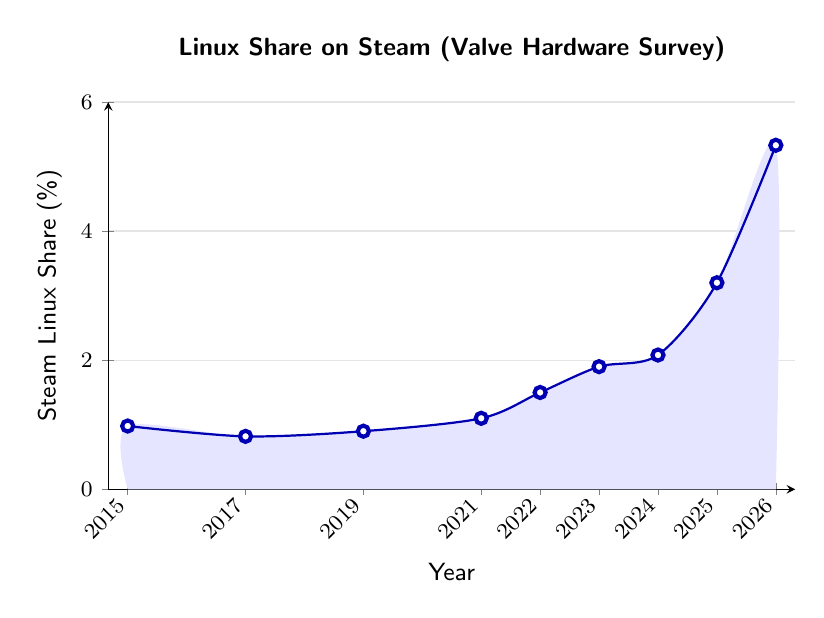
\begin{tikzpicture}
\begin{axis} [
    width=0.85\textwidth,
    height=6.5cm,
    title={\textbf{Linux Share on Steam (Valve Hardware Survey)}},
    title style={yshift=5pt, font=\small\sffamily},
    xlabel={Year},
    ylabel={Steam Linux Share (\%)},
    label style={font=\small\sffamily},
    xtick={2015,2017,2019,2021,2022,2023,2024,2025,2026},
    xticklabel style={rotate=45, anchor=east, font=\footnotesize\sffamily, /pgf/number format/1000 sep={}},
    yticklabel style={font=\footnotesize\sffamily},
    ymin=0, ymax=6,
    axis x line=bottom,
    axis y line=left,
    ymajorgrids=true,
    grid style={line width=0.5pt, draw=gray!20},
    enlarge x limits=0.03,
]


\addplot [
    draw=none,
    fill=blue!10,
    forget plot,
    smooth
] coordinates {
    (2015, 0) (2015, 0.98)
    (2017, 0.82)
    (2019, 0.90)
    (2021, 1.10)
    (2022, 1.50)
    (2023, 1.90)
    (2024, 2.08)
    (2025, 3.20)
    (2026, 5.33) (2026, 0)
};


\addplot [
    color=blue!70!black,
    thick,
    mark=*,
    mark options={fill=white, draw=blue!70!black, line width=1.5pt, mark size=2pt},
    smooth
] coordinates {
    (2015, 0.98)
    (2017, 0.82)
    (2019, 0.90)
    (2021, 1.10)
    (2022, 1.50)
    (2023, 1.90)
    (2024, 2.08)
    (2025, 3.20)
    (2026, 5.33)
};

\end{axis}
\end{tikzpicture}

\vspace{2mm}
{\footnotesize\sffamily\color{gray} Source: \href{https://steampowered.com}{Valve Steam Hardware \& Software Survey}}
\end{figure}



The release of the Steam Deck in 2022 accelerated this significantly. Running Valve's own \textit{SteamOS}, a Linux-based operating system, the Steam Deck proved that Linux could run a serious gaming library on consumer hardware. As of November 2025, \textit{Proton 10.0-3} is the latest stable release, bringing fixes and expanded support across thousands of titles including
\textit{God of War Ragnar\"{o}k}, \textit{Marvel's Spider-Man Remastered}, and more.

\begin{tcolorbox}[arc=12pt, outer arc=10pt,
  colback=blue!4!white, colframe=blue!40!black,
  title=\textbf{How Proton Works}]
  A Windows game makes calls to \textbf{DirectX} and the \textbf{Windows API}. \textit{Proton} intercepts these calls and translates them in real time using \textbf{DXVK} (DirectX $\rightarrow$ Vulkan) and \textbf{Wine} (Windows API $\rightarrow$ Linux). The game never knows it is not running on Windows.
\end{tcolorbox}

\noindent That said, Linux gaming is not without its caveats. Games with aggressive
kernel-level anti-cheat (such as Valorant's Vanguard or PUBG's BattlEye in certain configurations) remain the primary blocker. This is an active area of
development, and compatibility improves with every \textit{Proton} release.

\begin{tcolorbox}[arc=12pt, outer arc=10pt,
  colback=red!5!white, colframe=red!60!black,
  title=\textbf{Anti-Cheat Warning}]
  Before switching, check your most-played games on
  \href{https://www.protondb.com}{ProtonDB} and \href{https://areweanticheatyet.com}{areweanticheatyet.com}. Kernel-level anti-cheat is the one area where Linux genuinely cannot help you, yet.
\end{tcolorbox}

\newpage \section{Installing Linux}

This guide uses CachyOS as the recommended distribution.
\href{https://cachyos.org}{CachyOS} is an Arch-based rolling-release distribution that bundles all necessary gaming libraries, Proton, and dependencies into a single
meta-package install, making it one of the most convenient starting points for Linux gaming without sacrificing access to the full Arch ecosystem.
\begin{callout}{\textbf{Why Not Ubuntu or Fedora?}}
  Both are solid distros. CachyOS is chosen here purely for its convenience.
  One meta-package gets you a complete gaming setup. That is the only reason.
\end{callout}

\subsection{Choosing a Distro}

With hundreds of Linux distributions available, the choice can feel overwhelming. For
this guide, the decision has already been made: \textbf{CachyOS}. This subsection
explains why, and briefly covers the alternatives worth knowing about.

\subsubsection{Why CachyOS?}

\href{https://cachyos.org}{CachyOS} is an Arch-based rolling-release distribution. Its primary advantage for this guide is convenience: gaming libraries, Proton, and
all necessary dependencies are available as a single meta-package, meaning the gap between a fresh install and a working gaming setup is minimal.

Being Arch-based is also a practical advantage: Valve built SteamOS on Arch, meaning kernel-level fixes and gaming improvements from Valve tend to trickle down to
Arch-based distros like CachyOS naturally.

\subsubsection{Alternatives Worth Knowing}

CachyOS is not the only valid choice. The following are the most relevant alternatives:

\begin{itemize}[leftmargin=1.5em, label={\tiny\textbullet}, nosep]
  \item \textbf{Bazzite}: Fedora-based, immutable, excellent out-of-the-box gaming
    experience. Recommended for users who want something that simply works with minimal
    configuration. The safer choice for beginners.
  \item \textbf{Nobara}: Fedora-based, created by the developer of Proton-GE.
    Gaming tools pre-installed, good hardware support.
  \item \textbf{EndeavourOS}: Arch-based, minimal, close to vanilla Arch but with
    a friendlier installer. Less opinionated than CachyOS.
  \item \textbf{Ubuntu / Linux Mint}: Debian-based, highly stable, large community. Not gaming-optimized, but reliable and well-documented.
\end{itemize}

\begin{tcolorbox}[arc=12pt, outer arc=10pt,
  colback=blue!4!white, colframe=blue!40!black,
  title=\textbf{Rolling Release vs.\ Stable Release}]
  CachyOS is a \textbf{rolling release}, packages update continuously rather than
  in fixed version cycles. This means you always have the latest drivers and software,
  which matters for gaming. The trade-off is that updates occasionally introduce
  breakage. This guide covers basic troubleshooting for exactly that reason.
\end{tcolorbox}

\subsection{Preparing the Installation Medium}

Before Linux can be installed, a bootable installation medium must exist. Traditional tools such as \textit{Rufus} or \textit{balenaEtcher} flash a single ISO directly onto a USB drive; which works, but comes with a significant limitation: every time a different ISO is needed, the drive must be reformatted and rewritten from scratch.

\noindent This guide takes a different approach. Since a fallback Windows installer is useful to have on hand, in case anything goes wrong, both the CachyOS and Windows 11
ISOs will live on the same USB drive simultaneously. This is made possible by \textit{Ventoy}.

\href{https://www.ventoy.net}{Ventoy} installs a small bootloader onto the USB once.
After that, any number of ISO files can simply be copied onto the drive like normal
files. On boot, Ventoy presents a menu and lets you choose which ISO to launch.
No reflashing required.

\subsubsection{Downloads}

Before proceeding, download the following:

\begin{itemize}[nosep, leftmargin=1.5em, label={\tiny\textbullet}]
  \item \textbf{Ventoy} (Windows installer):
    \href{https://www.ventoy.net/en/download.html}{ventoy.net/en/download.html}
  \item \textbf{CachyOS Desktop Edition ISO}:
    \href{https://cachyos.org/download/}{cachyos.org/download}
  \item \textbf{Windows 11 Disk Image}:
    \href{https://www.microsoft.com/en-us/software-download/windows11}{microsoft.com}
\end{itemize}

\subsubsection{Installing Ventoy}

\begin{enumerate}[nosep, leftmargin=1.5em, label={\arabic*.}]
  \item Plug in your USB drive
  \item Extract the downloaded \code{Ventoy\_windows.zip} and open
    \code{Ventoy2Disk.exe}
  \item Your USB drive should appear in the device list
  \item Click Install, Ventoy will write its bootloader to the drive
  \item Once complete, open \directory{This PC} in Windows File Explorer
  \item Copy both ISO files directly onto the USB drive, no extraction needed
\end{enumerate}

\begin{tcolorbox}[arc=12pt, outer arc=10pt,
  colback=red!5!white, colframe=red!60!black,
  title=\textbf{Warning}]
  Installing Ventoy will erase all existing data on the USB drive. Back up anything important before proceeding. A USB drive of at least \textbf{16 GB} is recommended
  to fit both ISOs comfortably.
\end{tcolorbox}

\subsection{Booting into CachyOS}

With the USB prepared, the next step is to tell your PC to boot from it rather than the internal drive. This is done through the \textit{BIOS} or \textit{UEFI} firmware
settings, a low-level interface that controls hardware behaviour before the OS loads.

\subsubsection{Entering the BIOS}

\begin{enumerate}[leftmargin=1.5em, nosep, label={\arabic*.}]
  \item Plug in the USB drive
  \item Restart your PC
  \item As soon as the screen turns on, repeatedly press the BIOS entry key for your
    device. Common keys are \keys{F2}, \keys{Delete}, \keys{F10}, or \keys{F12}, the exact key varies by manufacturer and can be found with a quick search for your device model
\end{enumerate}

\begin{callout}{\textbf{Common BIOS Entry Keys by Manufacturer}}
  \begin{itemize}[leftmargin=1.5em, nosep, label={\tiny\textbullet}]
    \item \textbf{ASUS}: \keys{Delete} or \keys{F2}
    \item \textbf{MSI}: \keys{Delete}
    \item \textbf{Gigabyte}: \keys{Delete} or \keys{F2}
    \item \textbf{Dell}: \keys{F2} or \keys{F12}
    \item \textbf{HP}: \keys{F10} or \keys{Esc}
    \item \textbf{Lenovo}: \keys{F2} or \keys{Fn} + \keys{F2}
  \end{itemize}
\end{callout}

\subsubsection{Configuring Boot Order}

Once inside the BIOS:

\begin{enumerate}[leftmargin=1.5em, nosep, label={\arabic*.}]
 \item Navigate to a tab labelled \menu{Boot}, \menu{Boot Options}, or \menu{Boot Priority}, the exact name varies by firmware
  \item Move your USB device to the top of the boot order, above the internal drive
  \item Locate the Secure Boot option and set it to Disabled
  \item Press \keys{F10} to save and exit. Or navigate to \menu{Exit, Save Changes and Exit}
\end{enumerate}

\begin{tcolorbox}[arc=12pt, outer arc=10pt,
  colback=red!5!white, colframe=red!60!black,
  title=\textbf{Why Disable Secure Boot?}]
  Secure Boot is a firmware security feature that only allows signed bootloaders to
  run. While CachyOS supports Secure Boot, disabling it avoids potential complications
  during installation and is the recommended approach for a first-time Linux install.
  It can be re-enabled after setup if needed.
\end{tcolorbox}

\subsubsection{Selecting the CachyOS ISO in Ventoy}

After saving BIOS settings, your PC will restart and boot into the Ventoy menu:

\begin{enumerate}[leftmargin=1.5em, nosep, label={\arabic*.}]
  \item Use \keys{\arrowkeyup} and \keys{\arrowkeydown} to navigate to the CachyOS ISO
  \item Press \keys{\return} to boot into it
  \item CachyOS will load into a live environment, nothing is installed yet
\end{enumerate}

\subsection{The Installation Process}

With CachyOS booted from the Ventoy menu, the installation can begin. This subsection walks through every step of the Calamares installer sequentially, following the
\href{https://wiki.cachyos.org}{official CachyOS documentation}.

\subsubsection{Don't Panic; Boot Messages}\label{ssub:dont_panic}

As the ISO loads, you will likely see a screen full of rapidly scrolling white text on a black background. This is normal.  

\begin{mdframed}[linewidth=1.5pt, linecolor=black!50, topline=true, bottomline=true,
  leftline=false, rightline=false, backgroundcolor=black!3]
  \small\itshape
  ``Linux briefly displays system initialisation messages before the graphical desktop
  starts. Unlike Windows, which conceals this process behind splash screens and
  animations, Linux exposes it. These are kernel and \code{systemd} messages logged
  in real time as hardware is detected and services are started.''\\[4pt]
  \normalfont\small --- Behaviour described in the
  \href{https://wiki.archlinux.org/title/Systemd/Journal}{Arch Wiki: systemd/Journal}
  and \href{https://www.debian.org/doc/manuals/debian-reference/ch03.en.html}{Debian
  Reference, Chapter 3: System Initialisation}
\end{mdframed}

\noindent What you are seeing is \code{systemd}, the init system responsible for bootstrapping the user space after the kernel loads. When the kernel executes \code{systemd} as process 1, it takes over system initialisation,
orchestrating service startup, dependency tracking, and system management. Every line of text is a service starting, a device being detected, or a filesystem
being mounted. It looks chaotic. It is not.

The messages are produced by \code{systemd-journald}, the journal service that
logs both kernel and system messages, either into persistent binary
data below \directory{/var/log/journal} or into volatile binary data below
\directory{/run/log/journal/}. Once installed, you can review any boot's
messages at any time with: \begin{minted}{bash}
journalctl -b     # current boot messages
journalctl -b -1  # previous boot messages
\end{minted}


\begin{linuxterminal}
(*\graytext{Starting}*) Apply Kernel Variables...
(*\gbox{OK}*) Mounted Temporary /etc/pacman.d/gnupg directory.
(*\gbox{OK}*) Mounted Temporary directory /tmp.
(*\rbox{20.480467}*) vmwgfx 0000:00:02.0: [drm] (*\errtext{\string*ERROR\string*}*) vmwgfx seems to be running on an unsupported hypervisor.
(*\rbox{20.480475}*) vmwgfx 0000:00:02.0: [drm] (*\errtext{\string*ERROR\string*}*) This configuration is likely broken.
(*\rbox{20.480478}*) vmwgfx 0000:00:02.0: [drm] (*\errtext{\string*ERROR\string*}*) Please switch to a supported graphics device to avoid problems.
(*\gbox{OK}*) (*\graytext{Finished}*) Apply Kernel Variables.
(*\spc*) (*\graytext{Starting}*) Network Management...
(*\spc*) (*\graytext{Starting}*) Network Name Resolution...
(*\gbox{OK}*) Started Network Management.
(*\spc*) (*\graytext{Starting}*) Enable Persistent Storage in systemd-networkd...
(*\spc*) (*\graytext{Starting}*) Wait for Network to be Online...
(*\gbox{OK}*) Started Network Name Resolution.
(*\gbox{OK}*) (*\graytext{Reached target}*) Host and Network Name Lookups.
(*\gbox{OK}*) (*\graytext{Listening on}*) Load/Save RF Kill Switch Status /dev/rfkill Watch.
(*\spc*) (*\graytext{Starting}*) Virtual Console Setup...
(*\gbox{OK}*) Stopped Virtual Console Setup.
(*\spc*) (*\graytext{Starting}*) Virtual Console Setup...
(*\gbox{OK}*) (*\graytext{Finished}*) Enable Persistent Storage in systemd-networkd.
(*\gbox{OK}*) Stopped Virtual Console Setup.
(*\spc*) (*\graytext{Starting}*) Virtual Console Setup...
(*\gbox{OK}*) (*\graytext{Finished}*) Virtual Console Setup.
(*\gbox{OK}*) (*\graytext{Finished}*) Wait for udev To Complete Device Initialization.
(*\gbox{OK}*) (*\graytext{Reached target}*) ZFS pool import target.
(*\spc*) (*\graytext{Starting}*) Mount ZFS filesystems...
(*\gbox{OK}*) (*\graytext{Finished}*) Mount ZFS filesystems.
(*\gbox{OK}*) (*\graytext{Reached target}*) Local File Systems.
(*\gbox{OK}*) (*\graytext{Listening on}*) Boot Loader Control Service Socket.
(*\gbox{OK}*) (*\graytext{Listening on}*) System Extension Image Management.
(*\spc*) (*\graytext{Starting}*) Automatic Boot Loader Update...
(*\spc*) (*\graytext{Starting}*) Create System Files and Directories...
(*\spc*) (*\graytext{Starting}*) Load JSON user/group Records from Credentials...
(*\gbox{OK}*) (*\graytext{Finished}*) Automatic Boot Loader Update.
(*\gbox{OK}*) (*\graytext{Finished}*) Load JSON user/group Records from Credentials.
(*\gbox{OK}*) (*\graytext{Finished}*) Create System Files and Directories.
(*\spc*) (*\graytext{Starting}*) Rebuild Dynamic Linker Cache...
(*\spc*) (*\graytext{Starting}*) Initial Setup...
(*\spc*) (*\graytext{Starting}*) Rebuild Journal Catalog...
(*\spc*) (*\graytext{Starting}*) Record System Boot/Shutdown in UTMP...
(*\gbox{OK}*) (*\graytext{Finished}*) Record System Boot/Shutdown in UTMP.
(*\gbox{OK}*) (*\graytext{Finished}*) Initial Setup.
(*\gbox{OK}*) (*\graytext{Reached target}*) First Boot Complete.
(*\spc*) (*\graytext{Starting}*) Save Transient machine-id to Disk...
(*\gbox{OK}*) (*\graytext{Finished}*) Rebuild Journal Catalog.
(*\gbox{OK}*) (*\graytext{Finished}*) Save Transient machine-id to Disk.
(*\rbox{$\ast\ast\ast$}*) (3 of 3) A start job is running for Rebuild Dynamic Linker Cache (16s / no limit)
\end{linuxterminal}

\begin{multicols}{2}
\begin{center}
\begin{tabular}{@{}ll@{}}
\toprule
\textbf{Prefix} & \textbf{Meaning} \\
\midrule
\code{[  OK  ]} & Started successfully \\
\code{[ INFO ]} & Informational \\
\code{[~~~*~~~]} & Starting, wait \\
\bottomrule
\end{tabular}
\end{center}

\columnbreak

\begin{center}
\begin{tabular}{@{}ll@{}}
\toprule
\textbf{Prefix} & \textbf{Meaning} \\
\midrule
\code{[FAILED]} & Ignorable on live ISO \\
\code{[WARNING]} & Non-critical \\
\code{[DEPENDS]} & Waiting on another service \\
\bottomrule
\end{tabular}
\end{center}
\end{multicols}

\noindent Wait for the messages to finish. The graphical desktop will load
automatically. Once it does, you will be greeted by the \textbf{CachyOS Hello} window.

\begin{figure}[htbp]
  \centering
  \includegraphics[width=0.85\textwidth]{01.png}
  \caption*{\small\textit{CachyOS live desktop with Hello window on first boot}}
\end{figure}

\subsubsection{Network Connectivity}

Before launching the installer, a stable internet connection is required for the
online installation mode, which downloads the latest packages during install.

\begin{enumerate}[leftmargin=1.5em, nosep, label={\arabic*.}]
  \item Locate the \textbf{network tray icon} in the bottom-right corner of the taskbar
  \item Click it --- your available Wi-Fi networks will appear
  \item Select your network and enter your password
  \item Confirm connectivity before proceeding
\end{enumerate}

\begin{tcolorbox}[arc=12pt, outer arc=10pt,
  colback=red!5!white, colframe=red!60!black,
  title=\textbf{Warning}]
  Do not launch the installer on an unstable connection. If the download stalls at
  33\% progress, it is almost always a network issue --- not a system failure. The
  \href{https://wiki.cachyos.org/cachyos_basic/faq/}{official CachyOS FAQ} confirms this is the most common installation failure point.
\end{tcolorbox}

\noindent Once connected, click \textbf{Launch Installer} in the CachyOS Hello window. The Calamares installer will open.

\subsubsection{Language}

The first tab of Calamares asks for your preferred language. Select it from the list
and click \textbf{Next}.

\subsubsection{Timezone and Location}

Select your timezone from the map or the dropdown. This sets your system clock
correctly and determines locale defaults. Click \textbf{Next}.

\subsubsection{Keyboard Layout}

Select your keyboard layout. If you are unsure, the default for your selected region
is usually correct. Use the test field at the bottom of the screen to verify. Click
\textbf{Next}.

\subsubsection{Bootloader}

\begin{callout}{\textbf{What is a Bootloader?}}
  A bootloader is the software that runs before the operating system loads. It
  presents a menu where you select which OS to boot into. Windows has its own
  bootloader, \textbf{Windows Boot Manager}, but hides it behind splash
  screens. Linux exposes it directly and gives you the choice.
\end{callout}

\vspace{0.5em}

CachyOS offers two bootloader choices:

\begin{itemize}[leftmargin=1.5em, label={\tiny\textbullet}, nosep]
  \item \textbf{Limine} (recommended); a portable, modern bootloader and the
    reference implementation of the Limine boot protocol. According to the
    \href{https://wiki.cachyos.org/cachyos_basic/changelogs/gui_installer/}{CachyOS
    installer changelog}, Limine is now the default and ships with automatic Btrfs
    snapshot support out of the box
  \item \textbf{GRUB}, the GNU GRand Unified Bootloader, the traditional Linux
    standard. More compatible with dual-boot setups and older hardware, but does not
    offer automatic snapshot integration
\end{itemize}

\textbf{Choose Limine} for this guide and click \textbf{Next}.

\begin{callout}{\textbf{What are Snapshots?}}
  Snapshots are point-in-time copies of a filesystem. If a system update breaks
  something, you can boot a previous snapshot and restore your system to its last
  working state. Think of them as save states --- if something goes wrong, load the
  previous save.
\end{callout}

\subsubsection{Partitioning}

This guide assumes a full, dedicated Linux install, no dual boot. Select
\textbf{Erase Disk}.

\begin{tcolorbox}[arc=12pt, outer arc=10pt,
  colback=red!5!white, colframe=red!60!black,
  title=\textbf{Warning}]
  Erase Disk permanently deletes everything on the selected drive. Back up your
  Windows data before proceeding. Confirm you have selected the correct disk.
  If multiple drives are present, disconnect any you do not want wiped.
\end{tcolorbox}

\noindent After selecting Erase Disk, you will be prompted to choose a filesystem:

\begin{itemize}[leftmargin=1.5em, label={\tiny\textbullet}, nosep]
  \item \textbf{Btrfs} (recommended); supports snapshots natively. Combined with
    Limine, gives you automatic rollback capability. Calamares auto-detects whether
    your drive is an SSD or HDD and adjusts mount options accordingly
  \item \textbf{ext4}, the classic stable Linux filesystem. Widely supported, no
    snapshot capability
  \item \textbf{XFS}, high performance, good for large files, no snapshots
\end{itemize}

\begin{tcolorbox}[arc=12pt, outer arc=10pt,
  colback=blue!4!white, colframe=blue!40!black,
  title=\textbf{What is a Filesystem?}]
  A filesystem is the method by which an operating system organises and stores data
  on a drive. Linux supports multiple filesystems, Btrfs, ext4, XFS among others.
  Windows uses \textbf{NTFS}. Linux can read NTFS drives, but installing Linux itself
  on an NTFS partition is not supported or recommended.
\end{tcolorbox}

\noindent Select \textbf{Btrfs} and click \textbf{Next}.

\subsubsection{Desktop Environment}

\begin{tcolorbox}[arc=12pt, outer arc=10pt,
  colback=blue!4!white, colframe=blue!40!black,
  title=\textbf{Desktop Environment vs.\ Window Manager}]
  A \textbf{Desktop Environment} (DE) is a complete, integrated desktop experience ---
  file manager, settings app, notification tray, lock screen, and more, all packaged
  together. Think of it as a fully furnished house. Examples: KDE Plasma, GNOME, XFCE.\\[6pt]
  A \textbf{Window Manager} (WM) controls only window behaviour --- resizing, tiling,
  keyboard shortcuts. Think of it as the bare structure of a house with no furniture;
  you build everything yourself. Examples: Hyprland, niri, i3. Every DE ships with a
  WM already included --- KDE uses KWin, GNOME uses Mutter.
\end{tcolorbox}

\noindent For this guide, choose a Desktop Environment. Tiling window managers like
Hyprland are powerful but not appropriate for a first Linux install.

The available options for beginners:

\begin{itemize}[leftmargin=1.5em, label={\tiny\textbullet}, nosep]
  \item \textbf{KDE Plasma} (recommended): modern, feature-rich, highly
    customizable. Workflow is similar to Windows. The default choice for this guide
  \item \textbf{GNOME}: minimal, opinionated, clean. Closer in feel to macOS than
    Windows. A different workflow that takes adjustment
  \item \textbf{XFCE}: lightweight and efficient. Recommended only for older
    hardware with limited RAM
\end{itemize}

\begin{callout}{\textbf{Note}}
  There is no objectively best Desktop Environment. The difference is workflow.
  KDE is the starting point for most beginners due to its similarity to Windows and
  its depth of customization options. You are not locked in; CachyOS supports
  multiple DEs installed simultaneously, and you can switch later.
\end{callout}

\noindent Select \textbf{KDE Plasma} and click \textbf{Next}.

\begin{figure}[htbp]
  \centering
  \includegraphics[width=0.85\textwidth]{02.png}
  \caption*{\small\textit{Desktop Environment selection in Calamares}}
\end{figure}

\subsubsection{Packages}

Calamares will present a package selection screen. Ensure the default selections are
checked, these include the base KDE packages and essential system components.
Do not uncheck anything unless you know what you are removing. Click \textbf{Next}.

\subsubsection{Users}

Fill in the following fields:

\begin{itemize}[leftmargin=1.5em, nosep, label={\tiny\textbullet}, nosep]
  \item \textbf{Your name}: display name, can be anything
  \item \textbf{Username}: your login name, lowercase, no spaces
  \item \textbf{Computer name}: the hostname of your machine on the network
  \item \textbf{Password}: used for login and every \code{sudo} command. Do not
    forget this
\end{itemize}

\begin{tcolorbox}[arc=12pt, outer arc=10pt,
  colback=red!5!white, colframe=red!60!black,
  title=\textbf{Warning}]
  Your password is required for every administrative action on the system. There is
  no password recovery prompt like Windows --- if you forget it, recovery requires
  booting into a live environment and manually resetting it. Write it down somewhere
  safe.
\end{tcolorbox}

\subsubsection{Summary and Installation}

Calamares will display a full summary of your chosen configuration, language,
timezone, bootloader, filesystem, desktop, and username. Review everything carefully.
If anything is incorrect, use the \textbf{Back} button to correct it.

When satisfied, click \textbf{Install}. The installer will begin writing to disk.
Depending on your internet connection and drive speed, this takes between
\textbf{30 minutes and 2 hours}.

\begin{callout}{\textbf{During Installation}}
  Do not close the installer, put the machine to sleep, or disconnect from the
  internet while installation is in progress. An interrupted install can leave the
  drive in an unbootable state.
\end{callout}

\subsubsection*{What Happens During Installation}

At around 30\%, the copying of files is completed, this takes the longest. After
that, the installer creates users, removes live-system-specific packages, installs
additional packages, removes language packs and drivers not needed for your hardware,
and sets up the bootloader. On a network install, time depends entirely on your internet speed and mirror proximity.

\begin{callout}{\textbf{Progress Stages}}
  The progress bar is not linear. It will appear to stall. According to the \href{https://wiki.cachyos.org/cachyos_basic/faq/}{official CachyOS FAQ}, stalling
  at 33\% is almost always a network or mirror issue, not a system failure. Wait at
  least five minutes before concluding something is wrong.
\end{callout}

\subsubsection*{If Installation Fails}

If an installation fails, the installer may not properly unmount partitions, meaning continuous errors can occur if you attempt to reinstall
immediately. Always reboot back into the live ISO before trying again.

\subsubsection*{After Installation Completes}

When the installer finishes, Calamares will prompt you to restart. Remove the USB
drive when instructed and press \keys{\return}. Your system will boot into the
\textbf{Limine} bootloader menu, a clean interface showing your installed operating
systems. Select \textbf{CachyOS} and press \keys{\return}.

\noindent You are now running CachyOS. Section~3 covers what to do immediately
after first boot.

\begin{figure}[H]
\centering

% Define a sophisticated, cohesive color palette
\definecolor{nordBlue}{HTML}{5E81AC}
\definecolor{nordGreen}{HTML}{A3BE8C}
\definecolor{nordOrange}{HTML}{D08770}
\definecolor{gridGray}{HTML}{E5E9F0}
\definecolor{textDark}{HTML}{2E3440}
\definecolor{textMuted}{HTML}{4C566A}

% Ensure you have \usepackage{booktabs} and \usepackage{colortbl} in your preamble
\begin{tikzpicture}
\begin{polaraxis}[
    width=0.75\textwidth,
    % Configure clean, dashed background grids
    grid=both,
    grid style={line width=0.5pt, draw=gridGray, dashed},
    % Axis Limits and Ticks
    ymin=0, ymax=5,
    ytick={1,2,3,4,5},
    yticklabels={1,2,3,4,5},
    yticklabel style={font=\tiny\color{textMuted}, fill=white, inner sep=1pt},
    % Five-point star layout (360 / 5 = 72 degree increments)
    xtick={0, 72, 144, 216, 288},
    xticklabels={
        Snapshot\\Support,
        Raw\\Performance,
        Data\\Integrity,
        Stability,
        Recovery
    },
    % Multi-line text alignment for clear spacing
    xticklabel style={font=\small\color{textDark}, align=center, inner sep=8pt},
    % Clean, borderless horizontal legend placed cleanly underneath the chart
    legend style={
        at={(0.5,-0.15)},
        anchor=north,
        legend columns=-1,
        draw=none,
        fill=none,
        font=\small\color{textDark},
        /tikz/every even column/.append style={column sep=15pt}
    },
]

% --- Btrfs ---
\addplot[
    line width=1.5pt,
    color=nordBlue,
    fill=nordBlue,
    fill opacity=0.2,
    mark=*,
    mark size=2pt,
    mark options={fill=white, line width=1.5pt}
] coordinates {
    (0,   5)
    (72,  3)
    (144, 5)
    (216, 4)
    (288, 4)
    (360, 5)
};
\addlegendentry{Btrfs}

% --- ext4 ---
\addplot[
    line width=1.5pt,
    color=nordOrange,
    fill=nordOrange,
    fill opacity=0.2,
    mark=*,
    mark size=2pt,
    mark options={fill=white, line width=1.5pt}
] coordinates {
    (0,   0)
    (72,  5)
    (144, 3)
    (216, 5)
    (288, 4)
    (360, 0)
};
\addlegendentry{ext4}

% --- XFS ---
\addplot[
    line width=1.5pt,
    color=nordGreen,
    fill=nordGreen,
    fill opacity=0.2,
    mark=*,
    mark size=2pt,
    mark options={fill=white, line width=1.5pt}
] coordinates {
    (0,   0)
    (72,  5)
    (144, 3)
    (216, 5)
    (288, 3)
    (360, 0)
};
\addlegendentry{XFS}

\end{polaraxis}
\end{tikzpicture}

\vspace{8mm}

% Beautiful companion data table using booktabs structure
\small
\renewcommand{\arraystretch}{1.2} % Extra breathing room for rows
\begin{tabular}{lccccc}
    \toprule
    \color{textDark}Filesystem & Snapshot & Performance & Integrity & Stability & Recovery \\
    \midrule
    \color{nordBlue}Btrfs      & 5 & 3 & 5 & 4 & 4 \\
    \color{nordOrange}ext4     & 0 & 5 & 3 & 5 & 4 \\
    \color{nordGreen}XFS       & 0 & 5 & 3 & 5 & 3 \\
    \bottomrule
\end{tabular}

\vspace{6mm}
\begin{minipage}{0.85\textwidth}
    \centering
    {\fontsize{8.5pt}{11pt}\selectfont\color{textMuted}
    Qualitative comparison based on \href{https://linuxjournal.com}{Linux Journal},
    \href{https://linuxano.com}{Linuxano}, and \href{https://vps.do}{VPS.DO} filesystem
    analyses (2025--2026). Scores reflect desktop gaming use case priorities.\par}
\end{minipage}
\end{figure}

\subsection{Post-Install Checks}

The first boot into a fresh CachyOS install is not the time to start installing games.
Before anything else, the system needs to be verified, updated, and confirmed healthy.
Skipping these steps is how systems end up in broken states two weeks later.

\subsubsection{Update the System}

Open a terminal. On KDE Plasma, press \keys{META} or search for
\textbf{Konsole} in the application launcher. Run:

\begin{minted}{bash}
sudo pacman -Syu
\end{minted}

This synchronizes the package database and upgrades all installed packages. On a
fresh online install the list will be short. On an offline install, expect a
significantly larger download.

\begin{tcolorbox}[arc=12pt, outer arc=10pt,
  colback=red!5!white, colframe=red!60!black,
  title=\textbf{Warning}]
  Never run \code{pacman -Sy} or \code{pacman -Sy package} without the \code{u}
  flag. A partial upgrade on Arch-based systems introduces dependency
  mismatches that can break the entire system. Always use \code{-Syu}.
\end{tcolorbox}

\subsubsection{Verify paru; Your AUR Helper}

The \textbf{Arch User Repository} (AUR) is a community-maintained repository of
build scripts for software not available in the official Arch repositories. It is one
of the biggest practical advantages of using an Arch-based system. Nearly any
software you can think of has an AUR package.

To use the AUR, you need an \textbf{AUR helper}. CachyOS ships with
\href{https://github.com/morganamilo/paru}{\code{paru}}, a feature-rich AUR helper
written in Rust, installed by default. Confirm it is present:

\begin{minted}{bash}
paru --version
\end{minted}

If it prints a version number, \code{paru} is ready. If the terminal returns
\code{command not found}, install it manually:

\begin{minted}{bash}
sudo pacman -S --needed base-devel
git clone https://aur.archlinux.org/paru.git
cd paru
makepkg -si
\end{minted}

\begin{tcolorbox}[arc=12pt, outer arc=10pt,
  colback=blue!4!white, colframe=blue!40!black,
  title=\textbf{paru vs pacman}]
  \code{paru} is a wrapper around \code{pacman}. It handles everything \code{pacman}
  does, plus searches and builds AUR packages. The syntax is identical, anywhere
  you would use \code{pacman}, you can use \code{paru} instead. According to the
  \href{https://wiki.cachyos.org/cachyos_basic/faq/}{official CachyOS FAQ}, when AUR
  packages are installed, use \code{paru -Syu} for updates instead of \code{pacman
  -Syu} to ensure AUR packages are upgraded as well.
\end{tcolorbox}

\begin{callout}{\textbf{A Note on Graphical Package Managers}}
  The \href{https://wiki.cachyos.org/cachyos_basic/faq/}{official CachyOS FAQ}
  explicitly warns against using \textbf{Pamac} for system package management.
  It is known to improperly handle certain package management tasks, such as
  corrupting system keyrings, leading to PGP signature errors that prevent future
  updates. Use \code{pacman} or \code{paru} from the terminal for system updates.
\end{callout}

\subsubsection{Enable Multilib}

\textbf{Multilib} is a repository that provides 32-bit libraries on a 64-bit system.
It is required for Steam, many games, and Wine. On CachyOS it is typically enabled
by default, but verify it is active by opening the \directory{/etc/pacman.conf}:

\begin{minted}{bash}
sudo nano /etc/pacman.conf
\end{minted}

Scroll down and confirm the following lines are present and \textbf{uncommented}
(no \code{\#} at the start):

\begin{minted}{bash}
[multilib]
Include = /etc/pacman.d/mirrorlist
\end{minted}

If they are commented out, remove the \code{\#} characters, save with
\keys{Ctrl+O}, and exit with \keys{Ctrl+X}. Then sync:

\begin{minted}{bash}
sudo pacman -Syu
\end{minted}

\subsubsection{Verify GPU Drivers}

Before launching any games, confirm your GPU drivers are correctly loaded. Run:

\begin{minted}{bash}
	glxinfo | grep "OpenGL renderer"
\end{minted}

The output should display your GPU name, for example:

\begin{minted}{bash}
	OpenGL renderer string: NVIDIA GeForce RTX 3070/PCIe/SSE2
\end{minted}

\begin{tcolorbox}[arc=12pt, outer arc=10pt,
	colback=red!5!white, colframe=red!60!black,
	title=\textbf{Warning}]
	If the output shows \code{llvmpipe} or \code{softpipe}, the correct GPU drivers
	are not loaded. These are software renderers. Games will run at a fraction of
	their normal performance or not at all. Do not proceed to gaming setup until this
	is resolved.
\end{tcolorbox}

\noindent If \code{glxinfo} is not found, install it with:

\begin{minted}{bash}
	sudo pacman -S mesa-utils
\end{minted}

\subsubsection{Check Critical systemd Services}

Confirm that essential services are running correctly:

\begin{minted}{bash}
	systemctl --failed
\end{minted}

A healthy system returns an empty list. If any services appear as \code{failed},
investigate them individually:

\begin{minted}{bash}
	systemctl status service-name
\end{minted}

\begin{callout}{\textbf{NetworkManager}}
	The most common failed service on a fresh install is \code{NetworkManager}.
	If your network is working, it is running. This is sometimes a display artefact.
	Verify with:
	\begin{minted}{bash}
		systemctl status NetworkManager
	\end{minted}
	It should show \code{active (running)}.
\end{callout}

\noindent With the system updated, \code{paru} confirmed, multilib enabled, GPU
drivers verified, and services healthy, the system is ready. Section~3 covers
the first boot experience and initial desktop configuration.

%─────────────────────────────────────────────────────────────────────────────
\newpage
\section{First Boot}

You have successfully installed CachyOS. This section walks through the first boot
sequence, the login screen, and getting comfortable with your new desktop environment
before touching anything system-critical.

\subsection{The Limine Screen}

After removing the USB and rebooting, your system will present the \textbf{Limine}
bootloader menu. Use \keys{\arrowkeyup} and \keys{\arrowkeydown} to navigate to
\textbf{CachyOS} and press \keys{\return}.

\subsection{The Login Screen}

You will be greeted by a graphical login screen. This is the \textbf{display manager}
--- a program that provides a graphical login interface, handles user authentication,
and launches your chosen desktop environment.

\begin{tcolorbox}[arc=12pt, outer arc=10pt,
	colback=blue!4!white, colframe=blue!40!black,
	title=\textbf{What is a Display Manager?}]
	The display manager is the first graphical program that runs after boot. It starts
	the graphical environment, presents a login screen, authenticates the user, and
	then hands control to the desktop environment --- in this case, KDE Plasma. CachyOS
	uses \textbf{SDDM} (Simple Desktop Display Manager) by default.
\end{tcolorbox}

\noindent Type the password you set during installation and press \keys{\return}.

\subsection{Welcome to Linux}

CachyOS will greet you with the \textbf{CachyOS Hello} window --- a graphical tool
for post-install configuration, system tweaks, and package installation. You will
return to it later. For now, set it aside.

\subsection{Making Yourself at Home}

Before doing anything system-critical, spend a few minutes becoming comfortable
with the desktop. This is not wasted time --- familiarity with the UI makes
everything that follows easier.

\subsubsection{Changing the Wallpaper}

\begin{enumerate}[leftmargin=1.5em, nosep, label={\arabic*.}]
	\item Right-click on the desktop
	\item Select \menu{Desktop and Wallpaper} or press \keys{Ctrl+Shift+D}
	\item Choose a preloaded wallpaper, or add your own using the \textbf{Add} button
\end{enumerate}

\subsubsection{Customising the Panel}

\begin{enumerate}[leftmargin=1.5em, nosep, label={\arabic*.}]
	\item Right-click the bottom panel
	\item Select \menu{Show Panel Configuration}
	\item Adjust layout, widgets, and position to your preference
\end{enumerate}

\subsubsection{Things Worth Trying}

\begin{itemize}[leftmargin=1.5em, label={\tiny\textbullet}, nosep]
	\item Verify all keyboard shortcuts and keys are working. Customise them via
	\menu{System Settings, Shortcuts}
	\item Take a screenshot with \keys{PrtSc}
	\item Explore \menu{System Settings, Display and Monitor} to configure refresh
	rate and scaling
	\item Explore \menu{System Settings, Appearance} --- KDE ships with thousands
	of community-made themes, icon packs, and window decorations
\end{itemize}

\subsection{The Terminal}

On Linux, the terminal is not optional. It is the primary tool for system
administration, package management, and troubleshooting. A
\textbf{terminal emulator} is the graphical application that provides a window
for text input. Inside it runs a \textbf{shell}, the actual command interpreter
that reads your input and instructs the OS what to do.

\begin{tcolorbox}[arc=12pt, outer arc=10pt,
	colback=blue!4!white, colframe=blue!40!black,
	title=\textbf{Terminal vs.\ Shell}]
	The \textbf{terminal} is the window. The \textbf{shell} is the program running
	inside it. Common shells include \code{bash}, \code{zsh}, and \code{fish}.
	CachyOS uses \textbf{Fish} by default --- a user-friendly shell with
	autocompletion and syntax highlighting out of the box. The terminal emulator
	bundled with CachyOS is \textbf{Alacritty} --- a GPU-accelerated terminal
	built for speed.
\end{tcolorbox}

\noindent To open Alacritty, search for it in the application launcher. Pin it to
the taskbar, you will use it constantly. When Alacritty opens, you will see your system information displayed automatically.
This is \textbf{fastfetch} --- a pre-configured tool that prints a formatted system summary on terminal launch. Run it again at any time with:

\begin{minted}{bash}
	fastfetch
\end{minted}

\begin{figure}[H]
	\centering
	\includegraphics[width=0.85\textwidth]{03.png}
	\caption*{\small\textit{Alacritty terminal showing fastfetch system information output}}
\end{figure}



\begin{callout}{\textbf{Why fastfetch matters}}
	When asking for help on any Linux forum or subreddit, always include a screenshot
	of your fastfetch output. It tells others your distro, kernel version, DE, GPU,
	and RAM at a glance --- essential context for troubleshooting.
\end{callout}

%─────────────────────────────────────────────────────────────────────────────
\newpage
\section{File System}

Linux organises all files under a single unified directory tree rooted at \directory{/}.
Understanding this structure is essential --- knowing where configuration files, logs,
and game data live will save significant time when troubleshooting. This section covers
the official filesystem standard, the directory layout, and how to navigate it both
graphically and through the terminal.

\subsection{The Filesystem Hierarchy Standard}

Every file and directory on a Linux system lives under a single root directory:
\directory{/}. This structure is defined by the \textbf{Filesystem Hierarchy
	Standard} (FHS) --- a specification maintained by the Linux Foundation that defines
the directory layout and contents of Unix-like operating systems.

\begin{mdframed}[linewidth=1.5pt, linecolor=black!50, topline=true, bottomline=true,
	leftline=false, rightline=false, backgroundcolor=black!3]
	\small\itshape
	``This standard consists of a set of requirements and guidelines for file and
	directory placement under UNIX-like operating systems. The guidelines are intended
	to support interoperability of applications, system administration tools,
	development tools, and scripts as well as greater uniformity of these systems.''\\[4pt]
	\normalfont\small ---
	\href{https://refspecs.linuxfoundation.org/FHS_3.0/fhs/index.html}{Filesystem
		Hierarchy Standard 3.0, Linux Foundation}
\end{mdframed}

\noindent All files and directories appear under the root directory \directory{/}, even
if they are stored on different physical or virtual devices.  This is
fundamentally different from Windows, which assigns a drive letter (\directory{C:},
\directory{D:}) to each storage device. On Linux, everything is one unified tree.

\subsection{The Directory Tree}

\begin{minted}{bash}
	/
	├── bin/        # essential binaries (ls, cat, cp...)
	├── boot/       # kernel, initramfs, bootloader
	├── dev/        # device files (disks, USB, TTY...)
	├── etc/        # system-wide configuration files
	├── home/       # user home directories
	│   └── user/
	│       ├── Documents/
	│       ├── Downloads/
	│       └── ...
	├── lib/        # essential libraries for /bin
	├── media/      # auto-mounted removable drives
	├── mnt/        # manual mount points
	├── opt/        # optional/third-party software
	├── proc/       # virtual fs: live kernel & process info
	├── root/       # home directory of the root user
	├── run/        # runtime data (PIDs, sockets)
	├── srv/        # data for services (web, FTP...)
	├── sys/        # virtual fs: hardware & kernel info
	├── tmp/        # temporary files (cleared on reboot)
	├── usr/        # user utilities and applications
	│   ├── bin/    # most user commands live here
	│   ├── lib/    # libraries for /usr/bin
	│   ├── local/  # locally compiled software
	│   └── share/  # shared data (icons, docs, themes)
	└── var/        # variable data
	    ├── log/    # system logs
	    ├── cache/  # application cache
	    └── spool/  # print and mail queues
\end{minted}

{\footnotesize\color{gray} Structure defined by
	\href{https://refspecs.linuxfoundation.org/FHS_3.0/fhs/index.html}{FHS 3.0,
		Linux Foundation}. Identical across all FHS-compliant distributions.}

\begin{tcolorbox}[arc=12pt, outer arc=10pt,
	colback=blue!4!white, colframe=blue!40!black,
	title=\textbf{FHS 3.0}]
	The most recent version of the FHS, version 3.0, was published on March 18,
	2015, and is maintained by the Linux Foundation. Most Linux distributions are
	FHS-compliant, with the notable exception of NixOS, which uses a unique hierarchy
	built around the Nix package manager. 
\end{tcolorbox}
\subsection{Key Directories for Gamers}

Most of what you will interact with as a gamer lives in a small subset of these
directories:

\vspace{0.5em}
{\renewcommand{\arraystretch}{1.3}
	\begin{center}
		\begin{tabular}{@{}ll@{}}
			\toprule
			\textbf{Path} & \textbf{Relevance} \\
			\midrule
			\directory{/home/username/} & Your personal files, game saves, configs \\
			\directory{/home/username/.local/share/Steam} & Steam installation and game library \\
			\directory{/home/username/.steam} & Steam runtime and Proton data \\
			\directory{/etc/} & System-wide configuration files \\
			\directory{/var/log/} & System logs for troubleshooting \\
			\directory{/tmp/} & Temporary files, cleared on reboot \\
			\bottomrule
		\end{tabular}
\end{center}}

\begin{callout}{\textbf{Hidden Files}}
	Files and directories beginning with a \code{.} (dot) are hidden by default ---
	\directory{.steam}, \directory{.config}, \directory{.local}. They are not shown
	by \code{ls} unless you use \code{ls -a}. In Dolphin (KDE's file manager), press
	\keys{Ctrl+H} to toggle their visibility.
\end{callout}

\subsection{Navigating with the Terminal}

Open Alacritty and try the following in order. This is not a reference --- it is a
short walkthrough to build muscle memory.

Start by confirming where you are:

\begin{minted}{bash}
	pwd
\end{minted}

This will print \directory{/home/username} --- your home directory is the default
working directory every time a terminal opens. Now list everything in it:

\begin{minted}{bash}
	ls -a
\end{minted}

Your output will look similar to this:

\begin{minted}{text}
	.cache       .config      .local       .pki
	.var         Desktop      Documents    Downloads
	Music        Pictures     Projects     Public
	Templates    Videos       .bash_logout .bash_profile
	.bashrc      .gtkrc-2.0   .zshrc
\end{minted}

\noindent Entries beginning with \code{.} are hidden files and directories. Configuration
files, shell profiles, and application data. They are invisible by default in both
\code{ls} (without \code{-a}) and in Dolphin (without \keys{Ctrl+H}).

Now navigate into a subdirectory:

\begin{minted}{bash}
	cd Pictures/Screenshots
\end{minted}

\begin{callout}{\textbf{Tab Completion}}
	While typing any path, press \keys{Tab} to autocomplete. If multiple matches exist,
	press \keys{Tab} twice to see them all. Make this a habit --- it prevents typos and
	is significantly faster than typing full paths.
\end{callout}

Once inside \directory{Pictures/Screenshots}, list its contents:

\begin{minted}{bash}
	ls
\end{minted}

To open a file directly from the terminal, type its name. For an image file, your
default viewer will launch:

\begin{minted}{bash}
	xdg-open screenshot.png
\end{minted}

To return home at any point:

\begin{minted}{bash}
	cd ~
\end{minted}

\subsection{Navigating with Dolphin}

\textbf{Dolphin} is KDE's file manager and a capable graphical alternative to the
terminal for everyday file operations. Open it from the taskbar or application
launcher and spend a few minutes exploring --- copy, paste, rename, and move files
the same way you would on Windows.

Useful shortcuts:

\begin{itemize}[leftmargin=1.5em, nosep, label={\tiny\textbullet}]
	\item \keys{Ctrl+H} --- toggle hidden files and folders
	\item \keys{F4} --- open an embedded terminal panel at the current directory
	\item \keys{Ctrl+L} --- focus the path bar for direct path entry
	\item \keys{Alt+Left} / \keys{Alt+Right} --- navigate back and forward
\end{itemize}

\begin{callout}{\textbf{\keys{F4} is Underrated}}
	Pressing \keys{F4} in Dolphin opens a terminal panel locked to the directory you
	are currently browsing. This is the fastest way to drop into a terminal at a
	specific location without typing \code{cd} repeatedly.
\end{callout}

\subsubsection{Useful Commands}

The four commands you will use constantly:

\begin{minted}{bash}
	pwd          # print current working directory
	ls           # list directory contents
	ls -a        # list including hidden files
	cd Pictures  # change into the Pictures directory
	cd ~         # return to home directory
\end{minted}

\subsection{Launching Apps from the Terminal}

Every application on Linux can be launched by typing its name in the terminal:

\begin{minted}{bash}
	firefox     # launch Firefox and see its logs
	steam       # launch Steam with full log output
	vlc         # launch VLC
\end{minted}

This is more than a curiosity --- when an application crashes or behaves unexpectedly,
launching it from the terminal prints its log output in real time. This output is
often the fastest way to diagnose what went wrong, and is what Linux forums and
subreddits will ask you to provide when requesting help.
\newpage
\section{Terminal Basics}

The terminal is the most direct interface between you and the operating system. This
section covers command structure, essential commands, keyboard shortcuts, and piping
--- everything needed to operate confidently from the command line before moving into
package management and system configuration.

\subsection{Why the Terminal?}

Using a command-line interface provides unmatched speed, efficiency, and precise control over operations. While graphical tools exist for most tasks, the terminal is faster, scriptable, and always
available, even when the desktop environment breaks. On a rolling release distribution like CachyOS, knowing your way around the terminal is not optional.

\begin{mdframed}[linewidth=1.5pt, linecolor=black!50, topline=true, bottomline=true,
	leftline=false, rightline=false, backgroundcolor=black!3]
	\small\itshape
	``The shell is a command interpreter and programming language that provides the
	user interface to a Linux system. It interprets commands typed by the user
	and translates them into instructions the kernel can execute.''\\[4pt]
	\normalfont\small ---
	\href{https://www.gnu.org/software/bash/manual/bash.html}{GNU Bash Manual,
		gnu.org}
\end{mdframed}

\subsection{Anatomy of a Command}

Every command follows the same structure:

\begin{minted}{bash}
	command  [options]  [arguments]
\end{minted}

For example:

\begin{minted}{bash}
	ls  -la  /home/username
\end{minted}

Where \code{ls} is the command, \code{-la} are options (list all files in long
format), and \directory{/home/username} is the argument (the target directory).
Options beginning with a single dash (\code{-}) are short flags; those with double
dashes (\code{--}) are long-form equivalents:

\begin{minted}{bash}
	ls -a
	ls --all     # identical result
\end{minted}

% Define the Nord color palette
\definecolor{nordBlue}{HTML}{81A1C1}
\definecolor{nordOrange}{HTML}{D08770}
\definecolor{nordGreen}{HTML}{A3BE8C}

	
% Define the Nord color palette
\definecolor{nordBlue}{HTML}{81A1C1}
\definecolor{nordOrange}{HTML}{D08770}
\definecolor{nordGreen}{HTML}{A3BE8C}
\definecolor{nordDark}{HTML}{2E3440}
\definecolor{nordLight}{HTML}{D8DEE9}


	
\begin{center}
		\begin{tikzpicture}[
			box/.style={rounded corners=5pt, inner sep=8pt,
				font=\normalsize\ttfamily\bfseries, minimum width=2.0cm,
				minimum height=0.8cm, align=center},
			labelbox/.style={rounded corners=3pt, inner sep=5pt,
				font=\footnotesize\sffamily, minimum width=2.0cm,
				align=center},
			desc/.style={font=\scriptsize\sffamily\color{black!60},
				text width=2.6cm, align=center},
			arrow/.style={->, >=stealth, thick},
			terminal/.style={font=\small\ttfamily, color=black!70}
			]
			
			% --- LAYER 1: THE TERMINAL PROMPT & COMMAND ---
			% Prompt Prefix
			\node[terminal, anchor=east] (prompt) at (-1.5,0) {\textbf{\color{nordGreen}user@host}\color{black!50}{:}\textbf{\color{nordBlue}\raisebox{-0.5ex}{\~{}}}\color{black!70}{\$}};
			
			% Colored command boxes
			\node[box, fill=nordBlue!20, draw=nordBlue] (cmd) at (0,0) {ls};
			\node[box, fill=nordOrange!20, draw=nordOrange] (opt) at (3.2,0) {-la};
			\node[box, fill=nordGreen!20, draw=nordGreen] (arg) at (7.2,0) {/home/username};
			
			
			% --- LAYER 2: ANATOMY LABELS & DESCRIPTIONS ---
			% Labels
			\node[labelbox, fill=nordBlue!10, draw=nordBlue!40, text=nordBlue] (cmd-lbl) at (0,-1.3) {Command};
			\node[labelbox, fill=nordOrange!10, draw=nordOrange!40, text=nordOrange] (opt-lbl) at (3.2,-1.3) {Option};
			\node[labelbox, fill=nordGreen!10, draw=nordGreen!40, text=nordGreen] (arg-lbl) at (7.2,-1.3) {Argument};
			
			% Dynamic Arrows
			\draw[arrow, draw=nordBlue] (cmd.south) -- (cmd-lbl.north);
			\draw[arrow, draw=nordOrange] (opt.south) -- (opt-lbl.north);
			\draw[arrow, draw=nordGreen] (arg.south) -- (arg-lbl.north);
			
			% Descriptions
			\node[desc, anchor=north] at (cmd-lbl.south) {\vspace{0.1cm}The binary or program execution file};
			\node[desc, anchor=north] at (opt-lbl.south) {\vspace{0.1cm}Switches that modify tool behavior};
			\node[desc, anchor=north] at (arg-lbl.south) {\vspace{0.1cm}The target file, directory, or data};
			
			
			% --- LAYER 3: BRACKET & CONCEPT ---
			% Native TikZ Curly Brace
			\draw[decorate, decoration={calligraphic brace, amplitude=6pt}, thick, black!40]
			(-1.1, 0.6) -- (8.6, 0.6);
			\node[font=\footnotesize\sffamily\bfseries\color{black!60}, anchor=south] at (3.75, 0.9)
			{Input: Standard Execution String};
			
			
			% --- LAYER 4: COMMAND OUTPUT EXPLANATION (NEW) ---
			% Downward flow arrow to output
			\draw[arrow, black!20, line width=1.5pt] (3.75, -2.8) -- (3.75, -3.5);
			
			% Terminal Output Block
			\node[draw=black!20, fill=black!5, rounded corners=3pt, text width=10.5cm, font=\footnotesize\ttfamily, inner sep=10pt, anchor=north] (output) at (3.75, -3.6) {
				\color{black!50}{total 16} \\
				drwxr-xr-x  2 username username 4096 May 15 10:00 \color{nordBlue}{\textbf{.}} \\
				drwxr-xr-x  3 root     root     4096 May 15 09:00 \color{nordBlue}{\textbf{..}} \\
				-rw-r--r--  1 username username  220 May 15 09:00 .bash\_logout \\
				-rw-r--r--  1 username username 3771 May 15 09:00 .bashrc
			};
			
			% Output Label
			\node[font=\tiny\sffamily\color{black!40}, anchor=south east] at (output.south east) {Output (stdout)};
			
		\end{tikzpicture}
\end{center}


\subsection{Essential Commands}

\begin{minted}{bash}
	# Navigation
	pwd                    # print current directory
	cd /etc                # change to /etc
	cd ..                  # go up one directory
	cd ~                   # go to home directory
	
	# Files and directories
	ls -la                 # list all files with details
	mkdir myfolder         # create a directory
	rm file.txt            # delete a file
	rm -rf myfolder        # delete a directory recursively
	cp file.txt backup/    # copy a file
	mv file.txt docs/      # move a file
	cat file.txt           # print file contents
	
	# System
	sudo command           # run command as administrator
	man ls                 # open the manual for ls
	which firefox          # find where a binary lives
	echo $SHELL            # print your current shell
\end{minted}

\begin{tcolorbox}[arc=12pt, outer arc=10pt,
	colback=red!5!white, colframe=red!60!black,
	title=\textbf{Warning}]
	\code{rm -rf} is permanent and irreversible. There is no trash bin. Double-check
	the path before executing. Running \code{rm -rf /} as root deletes the entire
	filesystem. According to the
	\href{https://wiki.archlinux.org/title/Security}{Arch Wiki Security guide}, never
	run commands from the internet without reading and understanding them first.
\end{tcolorbox}

\subsection{Reading Manual Pages}

Every standard Linux command has a manual page:

\begin{minted}{bash}
	man pacman
\end{minted}

Navigate with \keys{\arrowkeyup}/\keys{\arrowkeydown}, search with \keys{/} followed
by a search term, and quit with \keys{q}.

\subsection{Useful Shortcuts}

\begin{center}
	{\renewcommand{\arraystretch}{1.3}
		\begin{tabular}{@{}ll@{}}
			\toprule
			\textbf{Shortcut} & \textbf{Action} \\
			\midrule
			\keys{Ctrl+C} & Kill the running process \\
			\keys{Ctrl+Z} & Suspend the running process \\
			\keys{Ctrl+D} & Exit the current shell session \\
			\keys{Ctrl+L} & Clear the terminal screen \\
			\keys{Tab}    & Autocomplete command or path \\
			\keys{\arrowkeyup} & Cycle through command history \\
			\keys{Ctrl+R} & Search command history interactively \\
			\bottomrule
	\end{tabular}}
\end{center}

\subsection{Pipes and Redirection}

Commands can be chained together using pipes (\code{|}) to pass output from one
command into another:

\begin{minted}{bash}
	# Find all running processes and search for steam
	ps aux | grep steam
	
	# Count lines in a file
	wc -l /var/log/pacman.log
	
	# Save command output to a file
	journalctl -b > boot_log.txt
\end{minted}

\begin{callout}{\textbf{A Note on Fish Shell}}
	CachyOS uses \textbf{Fish} as the default shell. Fish differs from \code{bash}
	in syntax for scripting (variables use \code{set} instead of \code{=}, for
	example), but for interactive use and the commands in this guide, the difference
	is invisible. If you copy \code{bash} scripts from the internet and they fail in
	Fish, run them explicitly with \code{bash script.sh}.
\end{callout}

%─────────────────────────────────────────────────────────────────────────────
\newpage
\section{Package Manager Basics}

On Linux, software does not come from scattered websites and \code{.exe} installers.
It comes from \textbf{repositories} --- curated, version-controlled collections of
packages maintained by the distribution team and the community. The package manager
is the tool that interfaces with these repositories: installing, upgrading, and
removing software with a single command, resolving dependencies automatically, and
keeping the entire system consistent. On CachyOS, that tool is \code{pacman},
supplemented by \code{paru} for the AUR.

\subsection{What is a Package Manager?}

A package manager is the tool that installs, upgrades, and removes software on your
system. Unlike Windows, where software is scattered across manufacturer websites and
installers, Linux centralises everything through repositories --- curated collections
of software maintained by the distribution team and the community.

\begin{mdframed}[linewidth=1.5pt, linecolor=black!50, topline=true, bottomline=true,
	leftline=false, rightline=false, backgroundcolor=black!3]
	\small\itshape
	``Pacman is a package management utility that tracks installed packages on a
	Linux system. It features dependency support, package groups, install and
	uninstall scripts, and the ability to sync your local machine with a remote
	repository to automatically upgrade packages.''\\[4pt]
	\normalfont\small ---
	\href{https://archlinux.org/pacman/pacman.8.html}{pacman man page, archlinux.org}
\end{mdframed}

\subsection{Where Packages Come From}

On CachyOS there are three sources, in order of preference:

\begin{enumerate}[leftmargin=1.5em, label={\arabic*.}, nosep]
	\item \textbf{Official repositories} --- packages maintained and tested by the
	Arch Linux team and CachyOS maintainers. Installed via \code{pacman}. Always
	prefer this source
	\item \textbf{AUR} (Arch User Repository) --- community-maintained build scripts
	for software not in official repos. Installed via \code{paru}. Verify the
	PKGBUILD before installing
	\item \textbf{Build from source} --- compile directly from a project's source code
	using \code{makepkg}. Use only when the above two options are unavailable
\end{enumerate}

\begin{callout}{\textbf{AUR Safety}}
	The AUR is community-maintained --- anyone can submit a package. According to the
	\href{https://wiki.cachyos.org/cachyos_basic/faq/}{CachyOS FAQ}, always read the
	PKGBUILD before installing an AUR package, and check the comment section for
	reported issues. Some packages are maintained by the software developers themselves
	(Google Chrome, Microsoft VS Code), which are generally safe.
\end{callout}

\begin{table}[h]
	\centering
	\small
	\caption{Overview of CachyOS Package Sources and Tools}
	\label{tab:package-managers}
	\vspace{0.5em} % Adds a small gap between caption and table
	\begin{NiceTabular}{lllll}[
		code-before = {
			\rowcolor{black!8}{1}
			\rowcolors{2}{white}{black!2}
		}
		]
		\toprule
		\textbf{Source} & \textbf{Tool} & \textbf{Maintained by} & \textbf{Safety} & \textbf{Speed} \\
		\midrule
		Official Repos & \code{pacman}   & Arch/CachyOS team & Highest         & Fastest \\
		AUR            & \code{paru}     & Community          & Moderate        & Fast    \\
		AUR            & \code{yay}      & Community          & Moderate        & Fast    \\
		Flatpak        & \code{flatpak}  & Flathub/Developers & High (Sandboxed)& Moderate\\
		Source         & \code{makepkg}  & You                & Verify yourself & Slowest \\
		\bottomrule
	\end{NiceTabular}
	\smallskip
	\begin{flushleft}
		\textit{Note: While \code{pacman} remains the core manager, \code{paru} and \code{yay} act as automated wrappers for the AUR. \code{Flatpak} provides an alternative, sandboxed layer, for desktop applications. }
	\end{flushleft}
\end{table}

\subsection{pacman Cheat Sheet}

\begin{minted}{bash}
	# Update system
	sudo pacman -Syu
	
	# Install a package
	sudo pacman -S vlc
	
	# Search for a package
	pacman -Ss vlc
	
	# Remove a package and its dependencies
	sudo pacman -Rns vlc
	
	# List installed packages
	pacman -Q
	
	# Search installed packages
	pacman -Qs vlc
	
	# Clean old package cache
	sudo pacman -Sc
	
	# Detailed info on installed package
	pacman -Qi vlc
	
	# Detailed info from remote repo
	pacman -Si vlc
	
	# Remove orphaned packages
	sudo pacman -Qdtq | pacman -Rns -
	
	# Clear entire cache (aggressive)
	sudo pacman -Scc
\end{minted}

\subsection{Installing from the AUR with paru}

\code{paru} uses identical syntax to \code{pacman}:

\begin{minted}{bash}
	# Install from AUR
	paru -S spotify
	
	# Update everything including AUR packages
	paru -Syu
	
	# Search AUR
	paru -Ss spotify
\end{minted}

\begin{tcolorbox}[arc=12pt, outer arc=10pt,
	colback=red!5!white, colframe=red!60!black,
	title=\textbf{Warning}]
	Avoid \textbf{Pamac} for system updates. The
	\href{https://wiki.cachyos.org/cachyos_basic/faq/}{official CachyOS FAQ}
	explicitly warns that Pamac is known to corrupt system keyrings on rolling-release
	systems, leading to PGP signature errors that block future updates. Use
	\code{pacman} or \code{paru} from the terminal.
\end{tcolorbox}

\subsection{Building from Source}

For software unavailable in official repos or the AUR, \code{makepkg} compiles
directly from source. This requires \code{base-devel}:

\begin{minted}{bash}
	# Install build tools
	sudo pacman -S --needed base-devel git
	
	# Clone the source repository
	git clone https://github.com/somedev/someproject
	cd someproject
	
	# Build and install
	makepkg -si
\end{minted}

\begin{callout}{\textbf{When to Build from Source}}
	Building from source is rarely necessary on CachyOS. The AUR covers the vast
	majority of software not in official repos. Resort to source builds only when no
	maintained AUR package exists or the AUR version is severely outdated.
\end{callout}

\newpage
\section{Permissions}

Every file and directory on a Linux system carries a set of permissions that controls
who can read it, write to it, or execute it. Understanding permissions is not optional
--- you will encounter them constantly when configuring the system, running scripts,
and troubleshooting access errors.

\subsection{The Three Permission Groups}

\begin{mdframed}[linewidth=1.5pt, linecolor=black!50, topline=true, bottomline=true,
	leftline=false, rightline=false, backgroundcolor=black!3]
	\small\itshape
	``chmod changes the file mode bits of each given file according to mode, which can
	be either a symbolic representation of changes to make, or an octal number
	representing the bit pattern for the new mode bits.''\\[4pt]
	\normalfont\small ---
	\href{https://www.gnu.org/software/coreutils/chmod}{GNU Coreutils Manual,
		gnu.org}
\end{mdframed}

\noindent According to the
\href{https://www.gnu.org/software/coreutils/chmod}{GNU Coreutils documentation},
every file on a Linux system has three permission groups:

\begin{itemize}[leftmargin=1.5em, label={\tiny\textbullet}, nosep]
	\item \textbf{Owner} (\code{u}): the user who created the file. Has the most
	control by default
	\item \textbf{Group} (\code{g}): every user belongs to one or more groups.
	When a file is created, it is assigned to the owner's primary group. Users in
	that group share the group permissions
	\item \textbf{Other} (\code{o}): every other user on the system who is neither
	the owner nor in the file's group
\end{itemize}

\noindent Each group can hold three permissions:

\begin{itemize}[leftmargin=1.5em, nosep, label={\tiny\textbullet}]
	\item \textbf{r} --- read: view file contents or list directory contents
	\item \textbf{w} --- write: modify a file or create/delete files inside a directory
	\item \textbf{x} --- execute: run a file as a program, or enter a directory
\end{itemize}

\subsection{Reading the Permission String}

Run the following in your terminal:

\begin{minted}{bash}
	ls -l
\end{minted}

\begin{minted}{bash}
	drwxr-xr-x
	││  │  │
	││  │  └── Other permissions (r-x)
	││  └───── Group permissions (r-x)
	│└──────── Owner permissions (rwx)
	└────────── Directory (d) or file (-)
\end{minted}

Each entry will show a permission string like this:

\begin{minted}{text}
	drwxr-xr-x  username  26 May 14:45  Downloads
\end{minted}

The first field, \code{drwxr-xr-x}, is the permission string. Here is how
to read it:

\begin{center}
	\begin{tikzpicture}[
		box/.style={rounded corners=3pt, inner sep=7pt,
			font=\small\ttfamily\bfseries, minimum height=0.75cm,
			minimum width=1.1cm, align=center},
		label/.style={font=\footnotesize\sffamily, align=center},
		desc/.style={font=\scriptsize\sffamily\color{black!60},
			text width=2.2cm, align=center},
		arrow/.style={->, >=stealth, thick, black!35}
		]
		\node[box, fill=black!8, draw=black!30] (type) at (0,0) {d};
		\node[box, fill=nordBlue!20, draw=nordBlue] (own) at (2.5,0) {rwx};
		\node[box, fill=nordOrange!20, draw=nordOrange] (grp) at (5,0) {r-x};
		\node[box, fill=nordGreen!20, draw=nordGreen] (oth) at (7.5,0) {r-x};
		
		\node[label] at (0,   -1.1) {Type};
		\node[label, text=nordBlue] at (2.5, -1.1) {Owner};
		\node[label, text=nordOrange] at (5,  -1.1) {Group};
		\node[label, text=nordGreen] at (7.5, -1.1) {Other};
		
		\draw[arrow, black!35]  (0,   -0.42) -- (0,   -0.72);
		\draw[arrow, nordBlue]  (2.5, -0.42) -- (2.5, -0.72);
		\draw[arrow, nordOrange](5,   -0.42) -- (5,   -0.72);
		\draw[arrow, nordGreen] (7.5, -0.42) -- (7.5, -0.72);
		
		\node[desc] at (0,   -2.0) {\code{d} = directory\\\code{-} = file};
		\node[desc] at (2.5, -2.0) {read, write,\\execute};
		\node[desc] at (5,   -2.0) {read, execute\\(no write)};
		\node[desc] at (7.5, -2.0) {read, execute\\(no write)};
	\end{tikzpicture}
\end{center}

\noindent So \code{drwxr-xr-x} means: this is a \textbf{directory}; the
\textbf{owner} can read, write, and enter it; the \textbf{group} can read and
enter it but not modify its contents; \textbf{others} have the same access as
the group.

\begin{callout}{\textbf{Execute on Directories}}
	The \code{x} permission on a directory does not mean running it as a program
	--- it means permission to \textit{enter} the directory and access files inside
	it. Without \code{x}, you cannot \code{cd} into a directory even if you can
	read it.
\end{callout}

\subsection{Modifying Permissions with \code{chmod}}

\code{chmod} (change mode) is the command used to modify file and directory
permissions. According to the
\href{https://www.gnu.org/software/coreutils/chmod}{GNU Coreutils manual}, only
the file's owner or a process with appropriate privileges (i.e.\ \code{sudo}) is
permitted to change its mode bits.

Syntax:

\begin{minted}{bash}
	chmod [mode] [file]
\end{minted}

There are two ways to express the mode: \textbf{symbolic} and \textbf{numeric}.

\subsubsection{Symbolic Mode}

Symbolic mode uses letters to specify who is affected and what changes:

\begin{center}
	{\renewcommand{\arraystretch}{1.25}
		\begin{tabular}{@{}ll@{}}
			\toprule
			\textbf{Symbol} & \textbf{Meaning} \\
			\midrule
			\code{u} & Owner (user) \\
			\code{g} & Group \\
			\code{o} & Other \\
			\code{a} & All (owner, group, and other) \\
			\midrule
			\code{+} & Add permission \\
			\code{-} & Remove permission \\
			\code{=} & Set exact permission \\
			\bottomrule
	\end{tabular}}
\end{center}

\vspace{0.5em}

Examples:

\begin{minted}{bash}
	# Give the owner execute permission
	chmod u+x file.txt
	
	# Give others read permission
	chmod o+r file.txt
	
	# Remove write permission from group
	chmod g-w file.txt
	
	# Give everyone read and execute, remove write
	chmod a=rx file.txt
\end{minted}

\subsubsection{Numeric Mode}

Numeric (octal) mode represents permissions as numbers. According to the
\href{https://manpages.debian.org/testing/coreutils/chmod.1.en.html}{Debian
	coreutils man page}, each permission type maps to a value:

\begin{center}
	{\renewcommand{\arraystretch}{1.25}
		\begin{tabular}{@{}lll@{}}
			\toprule
			\textbf{Permission} & \textbf{Symbol} & \textbf{Value} \\
			\midrule
			Read    & \code{r} & 4 \\
			Write   & \code{w} & 2 \\
			Execute & \code{x} & 1 \\
			None    & \code{-} & 0 \\
			\bottomrule
	\end{tabular}}
\end{center}

\vspace{0.5em}

\noindent Add the values together for each group to get a three-digit number:

\begin{minted}{text}
	rwx = 4+2+1 = 7
	r-x = 4+0+1 = 5
	r-- = 4+0+0 = 4
	rw- = 4+2+0 = 6
\end{minted}

So \code{drwxr-xr-x} from the earlier example becomes \code{755}:

\begin{minted}{bash}
	chmod 755 file.txt   # rwx for owner, r-x for group and other
	chmod 644 file.txt   # rw- for owner, r-- for group and other
\end{minted}

\begin{tcolorbox}[arc=12pt, outer arc=10pt,
	colback=blue!4!white, colframe=blue!40!black,
	title=\textbf{644 and 755 --- The Two You Will See Everywhere}]
	\textbf{644} (\code{rw-r--r--}) is the standard permission for files --- the
	owner can read and write, everyone else can only read. \textbf{755}
	(\code{rwxr-xr-x}) is the standard for directories and executables --- the
	owner has full access, everyone else can read and execute. These two appear
	constantly in Linux documentation and forum answers.
\end{tcolorbox}

\begin{callout}{\textbf{Numeric Mode is Not Optional Knowledge}}
	Representations like \code{755} and \code{644} appear throughout Linux
	documentation, forum answers, and configuration guides. Even if you prefer
	symbolic mode day-to-day, you need to be able to read and write numeric
	permissions fluently.
\end{callout}

\subsection{sudo --- Elevated Permissions}

Some files and directories are owned by \code{root}, the system administrator
account. Modifying them requires elevated privileges, granted by the \code{sudo}
command:

\begin{minted}{bash}
	sudo chmod 755 /etc/somefile
\end{minted}

\begin{tcolorbox}[arc=12pt, outer arc=10pt,
	colback=red!5!white, colframe=red!60!black,
	title=\textbf{Warning}]
	Do not run \code{chmod -R 777 /} or grant world-write permissions to system
	directories. \code{777} gives every user on the system full read, write, and
	execute access to a file --- a serious security risk. According to the
	\href{https://wiki.archlinux.org/title/Security}{Arch Wiki Security guide}, file
	permissions are a primary mechanism of Linux system security. Use the minimum
	permissions necessary.
\end{tcolorbox}

\newpage
\section{Shell Basics}

The terminal chapters so far have covered the practical side of using a terminal.
This section goes one level deeper --- what actually happens when a command is
run, and the different shells available on Linux.

\begin{tcolorbox}[arc=12pt, outer arc=10pt,
	colback=blue!4!white, colframe=blue!40!black,
	title=\textbf{Terminal vs.\ Shell, Revisited}]
	The \textbf{terminal} is the window through which you interact with the system.
	The \textbf{shell} is the program that actually interprets and executes what
	you type. They are related but distinct --- a single terminal emulator like
	Alacritty can run any shell inside it.
\end{tcolorbox}

\subsection{How a Shell Works}

The terminal acts as an input/output medium. When a command is entered:

\begin{minted}{bash}
	sudo pacman -Syu
\end{minted}

\noindent the shell parses the text, identifies the command and its arguments, and
asks the kernel to execute the corresponding program. This is a simplified
description, the shell does considerably more, including variable expansion,
job control, and scripting, but for practical day-to-day use, this is the
model worth carrying forward.

\subsection{Choosing a Shell}

Bash, Zsh, and Fish are the three most common shells on Linux. Each represents a
different point on the spectrum between stability/portability and modern
convenience.

\vspace{1em}

% Shell Spectrum Diagram
\begin{figure}[H]
	\centering
	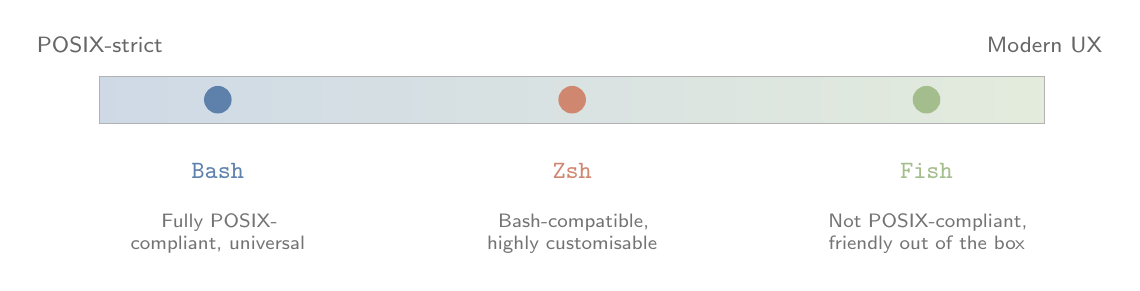
\begin{tikzpicture}[x=1cm]
		
		\definecolor{bashcol}{HTML}{5E81AC}
		\definecolor{zshcol}{HTML}{D08770}
		\definecolor{fishcol}{HTML}{A3BE8C}
		
		% Spectrum bar
		\shade[left color=bashcol!30, right color=fishcol!30]
		(0,0) rectangle (12,0.6);
		\draw[black!30] (0,0) rectangle (12,0.6);
		
		% Labels above bar
		\node[font=\footnotesize\sffamily\color{black!60}] at (0, 1.0) {POSIX-strict};
		\node[font=\footnotesize\sffamily\color{black!60}] at (12, 1.0) {Modern UX};
		
		% Shell markers
		\node[circle, fill=bashcol, minimum size=0.35cm, inner sep=0pt] (b) at (1.5, 0.3) {};
		\node[circle, fill=zshcol, minimum size=0.35cm, inner sep=0pt] (z) at (6, 0.3) {};
		\node[circle, fill=fishcol, minimum size=0.35cm, inner sep=0pt] (f) at (10.5, 0.3) {};
		
		% Shell name callouts below
		\node[font=\small\ttfamily\bfseries, text=bashcol] at (1.5, -0.6) {Bash};
		\node[font=\small\ttfamily\bfseries, text=zshcol] at (6, -0.6) {Zsh};
		\node[font=\small\ttfamily\bfseries, text=fishcol] at (10.5, -0.6) {Fish};
		
		\node[font=\scriptsize\sffamily\color{black!55}, text width=2.6cm, align=center]
		at (1.5, -1.4) {Fully POSIX-compliant, universal};
		\node[font=\scriptsize\sffamily\color{black!55}, text width=2.6cm, align=center]
		at (6, -1.4) {Bash-compatible, highly customisable};
		\node[font=\scriptsize\sffamily\color{black!55}, text width=2.8cm, align=center]
		at (10.5, -1.4) {Not POSIX-compliant, friendly out of the box};
		
	\end{tikzpicture}
	\caption*{\footnotesize\sffamily\color{gray}
		Shell positioning by POSIX compliance and default usability. Based on
		\href{https://www.gnu.org/software/bash/manual/html_node/index.html}{GNU
			Bash Manual} and
		\href{https://fishshell.com/docs/current/fish_for_bash_users.html}{Fish
			Shell official documentation}.}
\end{figure}

\subsubsection{Bash}

Bash (Bourne Again Shell) is the most widely used command-line shell and the
default on most Linux distributions.

\begin{mdframed}[linewidth=1.5pt, linecolor=black!50, topline=true, bottomline=true,
	leftline=false, rightline=false, backgroundcolor=black!3]
	\small\itshape
	Bash is highly compatible with Unix-like systems and is fully POSIX-compliant,
	which ensures that scripts written in Bash are portable and can run across
	different systems without issues.\\[4pt]
	\normalfont\small ---
	\href{https://www.gnu.org/software/bash/manual/html_node/index.html}{GNU Bash
		Reference Manual, gnu.org}
\end{mdframed}

\noindent Bash lacks some of the modern conveniences found in Fish or Zsh,
auto-suggestions and syntax highlighting are not built in, but it remains the
most stable, most documented, and most universally supported shell available.
Full documentation is at
\href{https://www.gnu.org/software/bash/manual/html_node/index.html}{gnu.org}.

\subsubsection{Zsh}

Zsh offers considerably more than Bash out of the box, advanced autocomplete,
extensive customisation, and a mature plugin ecosystem (most notably Oh My Zsh).
Zsh is also largely compatible with Bash scripts, so most existing Bash scripts
run without modification.

\begin{callout}{\textbf{More Features, More Complexity}}
	Zsh is not fully POSIX-compliant, it is closely compatible with Bash, but
	differs in edge cases. The trade-off for its extra features is a steeper
	learning curve, particularly once plugins and themes are involved.
\end{callout}

\subsubsection{Fish}

Fish (Friendly Interactive Shell) prioritises modern features and a user-friendly
interface, with many things that require manual configuration in Bash or Zsh
working out of the box, syntax highlighting, autosuggestions from history, and
sensible defaults.

\begin{tcolorbox}[arc=12pt, outer arc=10pt,
	colback=red!5!white, colframe=red!60!black,
	title=\textbf{Fish is Not POSIX-Compliant}]
	Fish is intentionally not POSIX-compliant. Bash scripts will not run correctly
	in Fish without modification, variable assignment, conditionals, and
	command substitution all use different syntax. According to the
	\href{https://fishshell.com/docs/current/fish_for_bash_users.html}{official
		Fish documentation}, this is a deliberate design choice, not an oversight.
\end{tcolorbox}

\noindent Fish ships with a built-in web-based configuration interface:

\begin{minted}{bash}
	fish_config
\end{minted}

\subsubsection{Which Shell Does CachyOS Use?}

\textbf{Fish} is the default shell on CachyOS, and most users are content to keep it. Shell choice is ultimately subjective, Bash for near-universal
support, Zsh for deep customisation, Fish for a friendly experience with minimal
setup.

\begin{callout}{\textbf{Why Bash Still Matters}}
	Even though Fish is the default, the majority of shell documentation, forum
	answers, wiki pages, and scripts found online are written in Bash. When
	searching for a fix or configuration tweak, the answer will almost always be
	in Bash syntax. Understanding Bash is not optional, it is the common
	language of the Linux ecosystem, regardless of which shell is used day to day.
\end{callout}

\noindent For that reason, whenever shell-specific syntax appears later in this
guide, Bash is covered first in full, with the Fish equivalent following as a
short note. Zsh is largely Bash-compatible and is not covered separately, Bash
examples apply directly.

\begin{tcolorbox}[arc=12pt, outer arc=10pt,
	colback=blue!4!white, colframe=blue!40!black,
	title=\textbf{A Useful Distinction}]
	\textbf{Shell syntax} (variable assignment, conditionals, loops) depends on
	which shell is being used. \textbf{Programs and commands} (\code{pacman},
	\code{ls}, \code{steam}) are shell-independent, they run identically no
	matter which shell invokes them.
\end{tcolorbox}

\newpage
\section{Environment Variables}

\subsection{What is an Environment Variable?}

An environment variable is a named value that a program reads when it starts.
In simple terms, it is a variable, a name paired with a value, that lives in the shell's environment and is passed down to any program launched from it.

Try the following:

\begin{minted}{bash}
	echo $HOME
	echo $USER
	echo $SHELL
	echo $PATH
\end{minted}

\noindent Each of these prints a value that programs on your system read
constantly, your home directory, your username, your default shell, and the
list of directories searched for executable programs.

\subsection{Checking Environment Variables}

To print every environment variable currently set, along with its value:

\begin{minted}{bash}
	printenv
\end{minted}

To check a single variable:

\begin{minted}{bash}
	echo $VAR
\end{minted}

\subsection{Why Environment Variables Matter}

Environment variables are used to pass data between processes and set global
defaults that applications read on startup. A few practical examples:

\begin{minted}{bash}
	USER=kunal              # specifies the current user, readable by any program
	SHELL=/bin/fish         # path to the default login shell
	GTK_THEME=Breeze-Dark firefox   # sets the theme Firefox uses for this session
	MANGOHUD=1 %command%    # enables the MangoHud overlay for a Steam game
\end{minted}

\noindent That last example should look familiar, it is the exact syntax used to enable MangoHud in Steam launch options, covered earlier in Section~\ref{sec:proton}. Environment variables are the mechanism behind that
entire feature.

\subsection{Setting Environment Variables --- By Scope}

Environment variables can be set at different scopes, from temporary
(a single command) to permanent (system-wide). The diagram below shows this as
a set of nested layers, from narrowest to broadest. Understanding these boundaries is crucial for avoiding configuration conflicts. When an application queries an environment variable, the operating system evaluates scopes from the inside out: it checks the immediate execution command environment first, falls back to the current shell session active state, searches the user profile configurations, and finally defaults to system-wide defaults. 

Consequently, narrower scopes always override broader ones. For instance, declaring a variable inline for a single command temporarily masks any identical system-wide configuration without permanently altering your system or shell profile properties.


\begin{figure}[H]
	\centering
	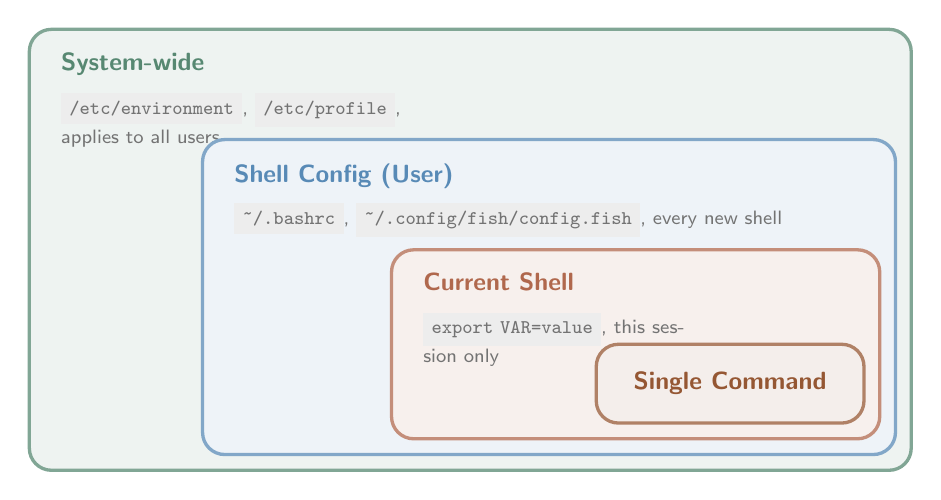
\begin{tikzpicture}[
		layer/.style={rounded corners=8pt, draw=#1!60, fill=#1!8, line width=1.2pt},
		lbl/.style={font=\small\sffamily\bfseries, text=#1!80, anchor=north west},
		sub/.style={font=\scriptsize\sffamily\color{black!55}, align=left, anchor=north west}
		]
		\definecolor{scopeA}{HTML}{7B2D00}
		\definecolor{scopeB}{HTML}{9C4221}
		\definecolor{scopeC}{HTML}{2E6DA4}
		\definecolor{scopeD}{HTML}{2D6A4F}
		
		% Outermost: System-wide
		\node[layer=scopeD, minimum width=11.2cm, minimum height=5.6cm] (sys) at (0,0) {};
		\node[lbl=scopeD] at ([xshift=0.3cm, yshift=-0.2cm]sys.north west) {System-wide};
		\node[sub, text width=4.8cm] at ([xshift=0.3cm, yshift=-0.7cm]sys.north west) {\code{/etc/environment}, \code{/etc/profile}, applies to all users};
		
		% User permanent
		\node[layer=scopeC, minimum width=8.8cm, minimum height=4.0cm] (usr) at (1.0,-0.6) {};
		\node[lbl=scopeC] at ([xshift=0.3cm, yshift=-0.2cm]usr.north west) {Shell Config (User)};
		% FIXED: Increased text width to 7.8cm to allow the long path to stretch horizontally
		\node[sub, text width=7.8cm] at ([xshift=0.3cm, yshift=-0.7cm]usr.north west) {\code{\textasciitilde/.bashrc}, \code{\textasciitilde/.config/fish/config.fish}, every new shell};
		
		% Current shell
		\node[layer=scopeB, minimum width=6.2cm, minimum height=2.4cm] (shell) at (2.1,-1.2) {};
		\node[lbl=scopeB] at ([xshift=0.3cm, yshift=-0.2cm]shell.north west) {Current Shell};
		\node[sub, text width=3.4cm] at ([xshift=0.3cm, yshift=-0.7cm]shell.north west) {\code{export VAR=value}, this session only};
		
		% Single command
		\node[layer=scopeA, minimum width=3.4cm, minimum height=1.0cm] (cmd) at (3.3,-1.7) {};
		\node[font=\small\sffamily\bfseries\color{scopeA!80}] at (cmd.center) {Single Command};
		
	\end{tikzpicture}
	\caption*{\footnotesize\sffamily\color{gray} Environment variable scope, from narrowest (a single command) to broadest (system-wide). Narrower scopes override broader ones.}
\end{figure}


\subsubsection{For a Single Command}

\begin{minted}{bash}
	EDITOR=nano git commit
\end{minted}

\noindent This sets \code{EDITOR} only for the duration of this one command.
Once it finishes, the variable is gone.

\subsubsection{For the Current Shell Session}

\begin{minted}{bash}
	export EDITOR=nano
\end{minted}

\begin{callout}{\textbf{What Does \texttt{export} Actually Do?}}
	\code{export} is a shell builtin that marks a variable as an environment
	variable, making it available to any program launched from the current shell.
	Without \code{export}, a variable exists only within the shell itself and is
	not passed down to child processes.
\end{callout}

\subsubsection{Permanently, Per-User}

Edit your shell's configuration file and add the export line:

\begin{itemize}[leftmargin=1.5em, nosep, label={\tiny\textbullet}]
	\item Fish: \directory{~/.config/fish/config.fish}
	\item Bash: \directory{~/.bashrc}
\end{itemize}

\noindent Add the line:

\begin{minted}{bash}
	export EDITOR=nano
\end{minted}

\noindent This variable is now set every time a new shell session starts.

\subsubsection{System-Wide, For All Users}

For variables that should apply regardless of which user or shell is in use,
define them in:

\begin{minted}{bash}
	/etc/environment
	/etc/profile
\end{minted}

\noindent These are permanent and system-wide, read before any user-specific shell configuration.

\subsubsection{Set by Applications}

Applications can also set environment variables for their own child processes.
The MangoHud example from earlier is exactly this, Steam sets
\code{MANGOHUD=1} for the single game process it launches:

\begin{minted}{bash}
	MANGOHUD=1 %command%
\end{minted}

\begin{tcolorbox}[arc=12pt, outer arc=10pt,
	colback=blue!4!white, colframe=blue!40!black,
	title=\textbf{Scope Overrides}]
	Narrower scopes take precedence over broader ones. A variable set for a single
	command overrides one exported in the current shell, which overrides one set
	in your shell config, which overrides a system-wide default. This layering is
	what allows per-game Steam launch options to override global settings without
	affecting anything else on the system.
\end{tcolorbox}

\newpage
\section{Services}

Most of what runs on a Linux distro does not run itself, it needs a
\textbf{service} to start it. The scrolling boot text covered in
Section~\ref{ssub:dont_panic} was \code{systemd} initialising exactly this,
starting every service, one by one, that a running system depends on.

\subsection{What Are Services and Daemons?}

\begin{mdframed}[linewidth=1.5pt, linecolor=black!50, topline=true, bottomline=true,
	leftline=false, rightline=false, backgroundcolor=black!3]
	\small\itshape
	What \code{systemd} calls a ``service'' was traditionally called a
	\textbf{daemon}: any program that runs as a background process, without a
	terminal or user interface, commonly waiting for events to occur and offering
	a service in response.\\[4pt]
	\normalfont\small ---
	Terminology as used throughout the
	\href{https://www.freedesktop.org/software/systemd/man/latest/systemd.service.html}{systemd.service(5)
		manual page, freedesktop.org}
\end{mdframed}

\subsection{What is systemd?}

\code{systemd} is a software suite for system and service management on Linux,
built to unify service configuration and behaviour across distributions.

\begin{tcolorbox}[arc=12pt, outer arc=10pt,
	colback=blue!4!white, colframe=blue!40!black,
	title=\textbf{PID 1}]
	As the first userspace process started by the Linux kernel, \code{systemd}
	runs as \textbf{PID 1}, process ID one. It is responsible for initialising
	the system and starting every service required for a functioning operating
	system. Every other process on the system is, directly or indirectly, a
	descendant of PID 1.
\end{tcolorbox}

\noindent Contrary to the traditional Unix philosophy of ``do one thing well,''
\code{systemd} is not limited to initialisation alone. According to its
\href{https://www.freedesktop.org/software/systemd/man/latest/systemd.html}{official
	manual}, it also provides device management, login management, network
connection management, and event logging --- functionality historically spread
across many separate, unrelated tools.

\subsection{Units}

\code{systemd} organises everything it manages into \textbf{units} --- objects
representing something systemd can start, stop, or monitor. A unit is defined by
a configuration file that tells systemd how to manage that object.

List all unit types systemd recognises:

\begin{minted}{bash}
	systemctl -t help
\end{minted}

\begin{minted}{text}
	Available unit types:
	service      mount        swap
	socket       target       device
	automount    timer        path
	slice        scope
\end{minted}

\noindent According to the
\href{https://man.archlinux.org/man/systemd.1.en}{official systemd manual page},
systemd manages exactly \textbf{11} unit types. This guide covers only
\textbf{service} units, by far the most relevant for everyday use.

\begin{callout}{\textbf{Naming Convention}}
	Service units carry a \code{.service} extension. Every service has a
	descriptive name, \code{NetworkManager.service}, \code{sshd.service},
	\code{bluetooth.service}. The name usually makes the service's purpose obvious.
\end{callout}

\subsection{Managing Services with \code{systemctl}}

\code{systemctl} is the command used to control and inspect service units.

\begin{minted}{bash}
	systemctl status <service>       # check if a service is running
	systemctl start <service>        # start a service (this boot only)
	systemctl stop <service>         # stop a running service
	systemctl restart <service>      # stop, then start again
	systemctl enable <service>       # start automatically on every boot
	systemctl disable <service>      # stop starting automatically
	systemctl enable --now <service> # enable AND start in one command
\end{minted}

\begin{tcolorbox}[arc=12pt, outer arc=10pt,
	colback=red!5!white, colframe=red!60!black,
	title=\textbf{Start vs.\ Enable --- Not the Same Thing}]
	\code{start} runs a service immediately, but it will not persist across a
	reboot. \code{enable} configures a service to start automatically on every
	future boot, but does \textit{not} start it right now. These are independent
	actions. To both start a service now and ensure it starts on every future
	boot, use \code{enable --now}.
\end{tcolorbox}

\subsection{Reading Logs with \code{journalctl}}

The \textbf{journal} is a unified log of everything managed by \code{systemd}.
\code{journalctl} is the tool used to inspect it.

\begin{minted}{bash}
	journalctl -u <service>       # full log history for one service
	journalctl -u <service> -f    # follow the log live, like tail -f
	journalctl -u <service> -b    # only entries from this boot
	journalctl -xe                # recent errors, system-wide
\end{minted}

\begin{callout}{\textbf{You Have Used This Already}}
	\code{journalctl -b} was introduced back in Section~\ref{ssub:dont_panic} to
	review boot messages. It is the same tool, now scoped to a specific
	service with \code{-u}.
\end{callout}

\subsection{Troubleshooting a Service}

When something is not working, a game controller not detected, Bluetooth not
connecting, Wi-Fi dropping, the issue is very often a failed or disabled
service. Work through the steps below in order:

\begin{callout}{\textbf{A Concrete Example}}
	Bluetooth headset not showing up in the device list? Nine times out of ten,
	the \code{bluetooth.service} is either not running or not enabled. Run
	\code{systemctl status bluetooth} first, if it shows \code{inactive} or
	\code{disabled}, that is very likely the entire problem, and the fix is a
	single command away.
\end{callout}

\vspace{1em}

\begin{figure}[H]
	\centering
	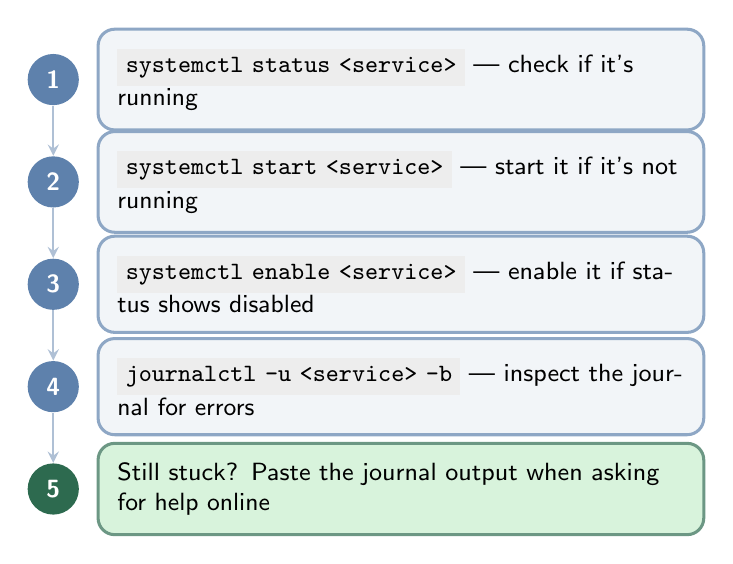
\begin{tikzpicture}[
		flowstep/.style={
			rounded corners=6pt, draw=nordBlue!70, fill=nordBlue!8,
			line width=1.1pt, font=\small\sffamily, inner sep=7pt,
			align=left, text width=7.2cm, minimum height=0.9cm
		},
		num/.style={
			circle, fill=nordBlue, text=white, font=\small\sffamily\bfseries,
			minimum size=0.65cm, inner sep=0pt
		},
		arrow/.style={->, >=stealth, thick, nordBlue!50}
		]
		
		\node[num] (n1) at (0, 0)    {1};
		\node[flowstep, anchor=west] (s1) at (0.55, 0)
		{\code{systemctl status <service>} --- check if it's running};
		
		\node[num] (n2) at (0, -1.3) {2};
		\node[flowstep, anchor=west] (s2) at (0.55, -1.3)
		{\code{systemctl start <service>} --- start it if it's not running};
		
		\node[num] (n3) at (0, -2.6) {3};
		\node[flowstep, anchor=west] (s3) at (0.55, -2.6)
		{\code{systemctl enable <service>} --- enable it if status shows disabled};
		
		\node[num] (n4) at (0, -3.9) {4};
		\node[flowstep, anchor=west] (s4) at (0.55, -3.9)
		{\code{journalctl -u <service> -b} --- inspect the journal for errors};
		
		\node[num, fill=moderngreen] (n5) at (0, -5.2) {5};
		\node[flowstep, anchor=west, draw=moderngreen!70, fill=moderngreenlight] (s5)
		at (0.55, -5.2)
		{Still stuck? Paste the journal output when asking for help online};
		
		\draw[arrow] (n1.south) -- (n2.north);
		\draw[arrow] (n2.south) -- (n3.north);
		\draw[arrow] (n3.south) -- (n4.north);
		\draw[arrow] (n4.south) -- (n5.north);
		
	\end{tikzpicture}
	\caption*{\footnotesize\sffamily\color{gray}
		General diagnostic flow for a misbehaving systemd service.}
\end{figure}

\begin{callout}{\textbf{Always Include the Journal Output}}
	When asking for help on any Linux forum or subreddit, the journal output from
	\code{journalctl -u <service> -b} is almost always the first thing you will
	be asked for. Include it upfront, it saves several rounds of back-and-forth
	and dramatically increases the odds of getting a useful answer.
\end{callout}

\newpage
\section{Setting Up NVIDIA Drivers and Gaming Packages}
\label{sec:nvidia}

Drivers are the software layer between the operating system and your GPU. Without
the correct driver loaded, the GPU runs on a generic fallback renderer; functional, but completely unsuitable for gaming. This section covers driver
installation for both AMD and NVIDIA GPUs, and explains the driver landscape
clearly so you can identify exactly what your hardware needs.

\subsection{AMD GPUs}

If you have an AMD GPU, the situation is straightforward.

\begin{mdframed}[linewidth=1.5pt, linecolor=black!50, topline=true, bottomline=true,
	leftline=false, rightline=false, backgroundcolor=black!3]
	\small\itshape
	The \texttt{amdgpu} kernel driver is the open-source AMD GPU driver maintained
	upstream in the Linux kernel. It supports all GCN and RDNA architecture cards
	and is included in the kernel by default --- no separate installation is required
	on a modern distribution like CachyOS.\\[4pt]
	\normalfont\small ---
	\href{https://wiki.archlinux.org/title/AMDGPU}{Arch Wiki: AMDGPU}
\end{mdframed}

\noindent Verify that the \code{amdgpu} driver is active:

\begin{minted}{bash}
	lspci -k | grep -A 3 VGA
\end{minted}

\noindent \code{lspci} lists all PCI devices. The \code{-k} flag shows which kernel driver
is in use for each device. \code{grep -A 3 VGA} filters the output to show only
the GPU entry and the three lines below it --- where the driver name appears. The
output should include:

\begin{minted}{text}
	Kernel driver in use: amdgpu
\end{minted}

\noindent If the driver is not loaded, install the required packages manually:

\begin{minted}{bash}
	sudo pacman -S mesa vulkan-radeon lib32-mesa lib32-vulkan-radeon
\end{minted}

\code{mesa} provides the OpenGL implementation. \code{vulkan-radeon} is the
Vulkan driver (required by most modern games and Proton). The \code{lib32-}
prefixed variants are the 32-bit equivalents, required by Steam and many games.

\begin{callout}{\textbf{AMD on Linux --- The Short Version}}
	AMD GPUs work out of the box on Linux because AMD has contributed their driver
	directly to the Linux kernel since 2014. There is no proprietary driver to
	install, no conflicts to manage, and no risk of a kernel update breaking your
	graphics. For gaming on Linux, AMD is the low-friction choice.
\end{callout}

\subsection{NVIDIA GPUs}

NVIDIA's driver situation on Linux is more complex. CachyOS ships with the
open-source \textbf{Nouveau} driver enabled by default, but Nouveau does not
support hardware acceleration for modern NVIDIA cards adequately ---
\href{https://wiki.archlinux.org/title/Nouveau}{the Arch Wiki} describes it as
suitable for basic desktop use only. For gaming, the proprietary NVIDIA driver
is required.

\begin{tcolorbox}[arc=12pt, outer arc=10pt,
	colback=blue!4!white, colframe=blue!40!black,
	title=\textbf{NVIDIA Driver Landscape (2025--2026)}]
	NVIDIA maintains multiple driver branches simultaneously. As of December 2025,
	\href{https://archlinux.org/news/nvidia-590-driver-drops-pascal-support-main-packages-switch-to-open-kernel-modules/}{Arch
		Linux officially announced} that the NVIDIA 590 driver dropped support for Pascal
	(GTX 10xx) and older architectures. Turing (RTX 20xx) and newer now use
	\code{nvidia-open} --- NVIDIA's partially open-source kernel module. Pascal and
	older must use legacy driver branches from the AUR.
\end{tcolorbox}

\subsubsection{Identifying Your GPU Architecture}

Before installing any driver, identify your GPU and its architecture:

\begin{minted}{bash}
	lspci | grep -i nvidia
\end{minted}

\begin{center}
	{\renewcommand{\arraystretch}{1.3}
		\definecolor{moderngreen}{HTML}{2D6A4F}
		\definecolor{moderngreenlight}{HTML}{D8F3DC}
		\definecolor{legacyorange}{HTML}{9C4221}
		\definecolor{legacyorangelight}{HTML}{FDEBD0}
		\definecolor{oldred}{HTML}{7B2D00}
		\definecolor{oldredlight}{HTML}{FDDCCA}
		\definecolor{timelineblue}{HTML}{2E6DA4}
		\begin{tabular}{@{}p{2.8cm}p{5.5cm}p{3cm}@{}}
			\toprule
			\textbf{Architecture} & \textbf{Example GPUs} & \textbf{Driver} \\
			\midrule
			\rowcolor{moderngreenlight}
			Blackwell   & RTX 5060, 5070, 5080, 5090          & \texttt{nvidia-open} \\
			\rowcolor{moderngreenlight}
			Ada Lovelace & RTX 4060, 4070, 4080, 4090          & \texttt{nvidia-open} \\
			\rowcolor{moderngreenlight}
			Ampere      & RTX 3050--3090, RTX 2050            & \texttt{nvidia-open} \\
			\rowcolor{moderngreenlight}
			Turing      & GTX 1650, 1660, RTX 2060--2080 Ti   & \texttt{nvidia-open}$^*$ \\
			\rowcolor{legacyorangelight}
			Volta       & Titan V                              & \texttt{nvidia-580xx-dkms} \\
			\rowcolor{legacyorangelight}
			Pascal      & GTX 1050--1080 Ti                   & \texttt{nvidia-580xx-dkms} \\
			\rowcolor{legacyorangelight}
			Maxwell     & GTX 750 Ti, 960--980 Ti             & \texttt{nvidia-580xx-dkms} \\
			\rowcolor{oldredlight}
			Kepler      & GTX 660, 680, 780 Ti                & \texttt{nvidia-470xx-dkms} \\
			\rowcolor{oldredlight}
			Fermi       & GTX 460, 560 Ti, 580                & \texttt{nvidia-390xx-dkms} \\
			\rowcolor{oldredlight}
			Tesla       & GTX 260, GTX 280                    & \texttt{nvidia-340xx-dkms} \\
			\bottomrule
			\multicolumn{3}{@{}l@{}}{\scriptsize $^*$ Some Turing cards may need
				\texttt{nvidia-580xx-dkms} for power management --- see note below.}
	\end{tabular}}
\end{center}



\noindent This prints your GPU model name. Use the timeline below to locate your
architecture and identify the correct driver branch:

\vspace{1em}

% GPU Architecture Timeline
\begin{figure}[H]
	\centering
	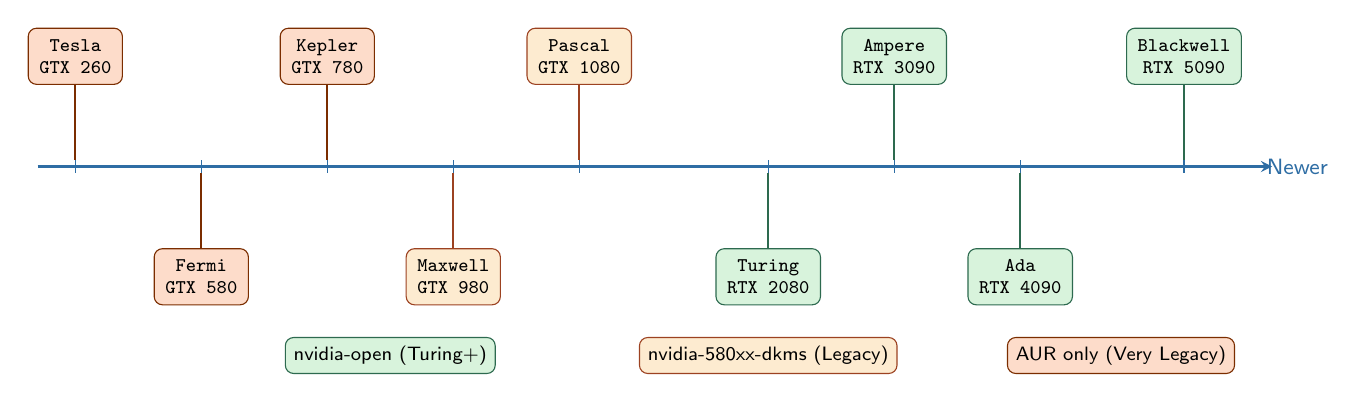
\begin{tikzpicture}[x=1.6cm]
		
		% Color definitions
		\definecolor{moderngreen}{HTML}{2D6A4F}
		\definecolor{moderngreenlight}{HTML}{D8F3DC}
		\definecolor{legacyorange}{HTML}{9C4221}
		\definecolor{legacyorangelight}{HTML}{FDEBD0}
		\definecolor{oldred}{HTML}{7B2D00}
		\definecolor{oldredlight}{HTML}{FDDCCA}
		\definecolor{timelineblue}{HTML}{2E6DA4}
		
		% Timeline axis
		\draw[thick, timelineblue, ->, >=stealth] (-0.3,0) -- (9.5,0);
		\node[font=\footnotesize\sffamily\color{timelineblue}]
		at (9.7, 0) {Newer};
		
		% --- Nodes ---
		% Tesla
		\node[draw=oldred, fill=oldredlight, rounded corners=3pt,
		font=\scriptsize\ttfamily, inner sep=4pt, align=center]
		(tesla) at (0, 1.4) {Tesla\\GTX 260};
		\draw[oldred, thick] (0,0.08) -- (0,1.05);
		
		% Fermi
		\node[draw=oldred, fill=oldredlight, rounded corners=3pt,
		font=\scriptsize\ttfamily, inner sep=4pt, align=center]
		(fermi) at (1, -1.4) {Fermi\\GTX 580};
		\draw[oldred, thick] (1,-0.08) -- (1,-1.05);
		
		% Kepler
		\node[draw=oldred, fill=oldredlight, rounded corners=3pt,
		font=\scriptsize\ttfamily, inner sep=4pt, align=center]
		(kepler) at (2, 1.4) {Kepler\\GTX 780};
		\draw[oldred, thick] (2,0.08) -- (2,1.05);
		
		% Maxwell
		\node[draw=legacyorange, fill=legacyorangelight, rounded corners=3pt,
		font=\scriptsize\ttfamily, inner sep=4pt, align=center]
		(maxwell) at (3, -1.4) {Maxwell\\GTX 980};
		\draw[legacyorange, thick] (3,-0.08) -- (3,-1.05);
		
		% Pascal
		\node[draw=legacyorange, fill=legacyorangelight, rounded corners=3pt,
		font=\scriptsize\ttfamily, inner sep=4pt, align=center]
		(pascal) at (4, 1.4) {Pascal\\GTX 1080};
		\draw[legacyorange, thick] (4,0.08) -- (4,1.05);
		
		% Turing
		\node[draw=moderngreen, fill=moderngreenlight, rounded corners=3pt,
		font=\scriptsize\ttfamily, inner sep=4pt, align=center]
		(turing) at (5.5, -1.4) {Turing\\RTX 2080};
		\draw[moderngreen, thick] (5.5,-0.08) -- (5.5,-1.05);
		
		% Ampere
		\node[draw=moderngreen, fill=moderngreenlight, rounded corners=3pt,
		font=\scriptsize\ttfamily, inner sep=4pt, align=center]
		(ampere) at (6.5, 1.4) {Ampere\\RTX 3090};
		\draw[moderngreen, thick] (6.5,0.08) -- (6.5,1.05);
		
		% Ada
		\node[draw=moderngreen, fill=moderngreenlight, rounded corners=3pt,
		font=\scriptsize\ttfamily, inner sep=4pt, align=center]
		(ada) at (7.5, -1.4) {Ada\\RTX 4090};
		\draw[moderngreen, thick] (7.5,-0.08) -- (7.5,-1.05);
		
		% Blackwell
		\node[draw=moderngreen, fill=moderngreenlight, rounded corners=3pt,
		font=\scriptsize\ttfamily, inner sep=4pt, align=center]
		(blackwell) at (8.8, 1.4) {Blackwell\\RTX 5090};
		\draw[moderngreen, thick] (8.8,0.08) -- (8.8,1.05);
		
		% Tick marks on axis
		\foreach \x in {0,1,2,3,4,5.5,6.5,7.5,8.8}
		\draw[timelineblue] (\x, 0.08) -- (\x, -0.08);
		
		% Legend
		\node[draw=moderngreen, fill=moderngreenlight, rounded corners=3pt,
		font=\scriptsize\sffamily, inner sep=3pt] at (2.5, -2.4)
		{nvidia-open (Turing+)};
		\node[draw=legacyorange, fill=legacyorangelight, rounded corners=3pt,
		font=\scriptsize\sffamily, inner sep=3pt] at (5.5, -2.4)
		{nvidia-580xx-dkms (Legacy)};
		\node[draw=oldred, fill=oldredlight, rounded corners=3pt,
		font=\scriptsize\sffamily, inner sep=3pt] at (8.3, -2.4)
		{AUR only (Very Legacy)};
		
	\end{tikzpicture}
	\caption*{\footnotesize\sffamily\color{gray}
		Driver branches per architecture. Source:
		\href{https://archlinux.org/news/nvidia-590-driver-drops-pascal-support-main-packages-switch-to-open-kernel-modules/}{Arch
			Linux News, December 2025} and
		\href{https://wiki.cachyos.org}{wiki.cachyos.org}}
\end{figure}

\subsubsection{Installing NVIDIA Drivers}

\paragraph{Turing, Ampere, Ada Lovelace, Blackwell (RTX 20xx and newer):}

\begin{minted}{bash}
	sudo pacman -S linux-cachyos-nvidia-open
	sudo pacman -S nvidia-utils lib32-nvidia-utils nvidia-settings
\end{minted}

\noindent \code{linux-cachyos-nvidia-open} is the CachyOS-patched NVIDIA open kernel module,
pre-built for the CachyOS kernel. \code{nvidia-utils} provides user-space utilities
including \code{nvidia-smi}. \code{lib32-nvidia-utils} provides 32-bit support
required by Steam. \code{nvidia-settings} is the graphical driver configuration tool.

\begin{callout}{\textbf{Turing Power Management}}
	Some Turing cards (RTX 20xx) experience power management issues with
	\code{nvidia-open}. If your system fails to suspend, resume, or experiences
	instability, switch to the legacy proprietary branch instead:
	\begin{minted}{bash}
		paru -S nvidia-580xx-dkms
	\end{minted}
\end{callout}

\paragraph{Maxwell, Pascal (GTX 900, GTX 10xx):}

\begin{minted}{bash}
	paru -S nvidia-580xx-dkms
\end{minted}

\noindent \code{nvidia-580xx-dkms} is the last driver branch supporting Maxwell and Pascal.
It is in the AUR rather than official repos because, as of December 2025,
\href{https://archlinux.org/news/nvidia-590-driver-drops-pascal-support-main-packages-switch-to-open-kernel-modules/}{Arch
	Linux dropped Pascal and older from the official NVIDIA packages}. \code{dkms}
means the driver rebuilds itself automatically against new kernels.

\paragraph{Kepler (GTX 600, GTX 700):}

\begin{minted}{bash}
	paru -S nvidia-470xx-dkms
\end{minted}

\paragraph{Fermi (GTX 400, GTX 500):}

\begin{minted}{bash}
	paru -S nvidia-390xx-dkms
\end{minted}

\paragraph{Tesla (GTX 200):}

\begin{minted}{bash}
	paru -S nvidia-340xx-dkms
\end{minted}

\begin{tcolorbox}[arc=12pt, outer arc=10pt,
	colback=red!5!white, colframe=red!60!black,
	title=\textbf{Reboot Required}]
	After installing any NVIDIA driver, reboot before proceeding. The driver is not
	active until the system restarts and loads the new kernel module. Running games
	or verifying the driver before rebooting will produce incorrect results.
\end{tcolorbox}

\subsubsection{Verifying the NVIDIA Driver}

After rebooting, confirm the driver is loaded correctly:

\begin{minted}{bash}
	nvidia-smi
\end{minted}

\noindent \code{nvidia-smi} (System Management Interface) is a tool provided by
\code{nvidia-utils} that queries the NVIDIA driver directly. A successful output
displays your GPU model, the loaded driver version, VRAM usage, and running
processes. If the command returns \code{command not found} or an error, the
driver did not load correctly --- check \code{journalctl -b} for error messages
related to \code{nvidia}.

\begin{callout}{\textbf{Double-Check the Driver Version}}
	Confirm the driver version shown by \code{nvidia-smi} matches the package you
	installed. A mismatch between the kernel module version and \code{nvidia-utils}
	version causes errors. If they differ, run \code{sudo pacman -Syu} to
	synchronise everything.
\end{callout}

\newpage
\section{Preparing and Gaming Environment}

Steam is the primary gaming platform on Linux, and Proton is the engine that makes
the majority of its library playable. This section covers installing the essential
gaming packages, setting up Steam, and configuring Proton correctly.

\subsection{Installing Gaming Packages}

The fastest way to install all essential gaming packages on CachyOS is through
\textbf{CachyOS Hello}:

\begin{enumerate}[leftmargin=1.5em, nosep, label={\arabic*.}]
	\item Open \textbf{CachyOS Hello} from the application launcher
	\item Navigate to the \textbf{Tweaks} tab
	\item Locate \textbf{Install Gaming Packages} and run it
\end{enumerate}

This installs \code{cachyos-gaming-meta} and \code{cachyos-gaming-applications} in
a single click. Steam, Lutris, Heroic, Bottles, Proton, Wine, MangoHud, GameMode,
and all required libraries included.

\begin{callout}{\textbf{Prefer the Minimal Route?}}
	If you prefer a manual install without CachyOS Hello, run the following instead:
	\begin{minted}{bash}
		sudo pacman -S steam gamemode lib32-gamemode \
		mangohud lib32-mangohud wine winetricks \
		lutris protonup-qt vulkan-tools
		paru -S heroic-games-launcher-bin
	\end{minted}
	This installs the same core tools individually. The backslash \code{\textbackslash}
	continues a long command across multiple lines --- the shell treats it as one
	command.
\end{callout}

\subsection{What is Proton?}

\begin{mdframed}[linewidth=1.5pt, linecolor=black!50, topline=true, bottomline=true,
	leftline=false, rightline=false, backgroundcolor=black!3]
	\small\itshape
	``Proton is a compatibility layer that allows Windows software (primarily video
	games) to run on Linux-based operating systems. Proton is developed by Valve
	in cooperation with developers from CodeWeavers.''\\[4pt]
	\normalfont\small ---
	\href{https://en.wikipedia.org/wiki/Proton_(software)}{Wikipedia: Proton
		(software)}, sourced from
	\href{https://github.com/ValveSoftware/Proton}{ValveSoftware/Proton, GitHub}
\end{mdframed}

\noindent Proton is developed by Valve in cooperation with CodeWeavers. Its stable
release as of November 2025 is Proton 10.0-3.  It is a fork of
\textbf{Wine}, a compatibility layer that translates Windows API calls into
POSIX-compliant equivalents, extended with additional components specifically
for gaming performance and compatibility. Proton is a runtime translator rather than a hardware emulator, decoupling Windows games from Microsoft Windows by unifying several open-source graphic compilation projects. Its core components are:

\begin{itemize}[leftmargin=1.5em, nosep, label={\tiny\textbullet}]
	\item \textbf{DXVK (DirectX 9/10/11 to Vulkan):} Translates Direct3D API commands and shader structures into Vulkan API calls, reducing rendering latency on Linux hardware.
	\item \textbf{VKD3D-Proton (DirectX 12 to Vulkan):} A fork of Wine's VKD3D that maps Direct3D 12 features—including raytracing, mesh shaders, and binding models—directly into native Vulkan.
	\item \textbf{Wine-Mono:} An open-source .NET framework implementation that runs managed game engines and launchers within the Linux workspace.
	\item \textbf{Custom Synchronization Patches (Fsync):} Kernel-level additions that replace Wine's legacy server lock bottlenecks with event-driven system handles to improve multicore scaling.
\end{itemize}

When a Windows executable runs, graphic calls route to Vulkan, execution threads use POSIX thread abstractions, and inputs map to the host desktop environment. This architecture ensures near-native performance, as shown in the metrics below.

\begin{figure}[H]
	\centering
	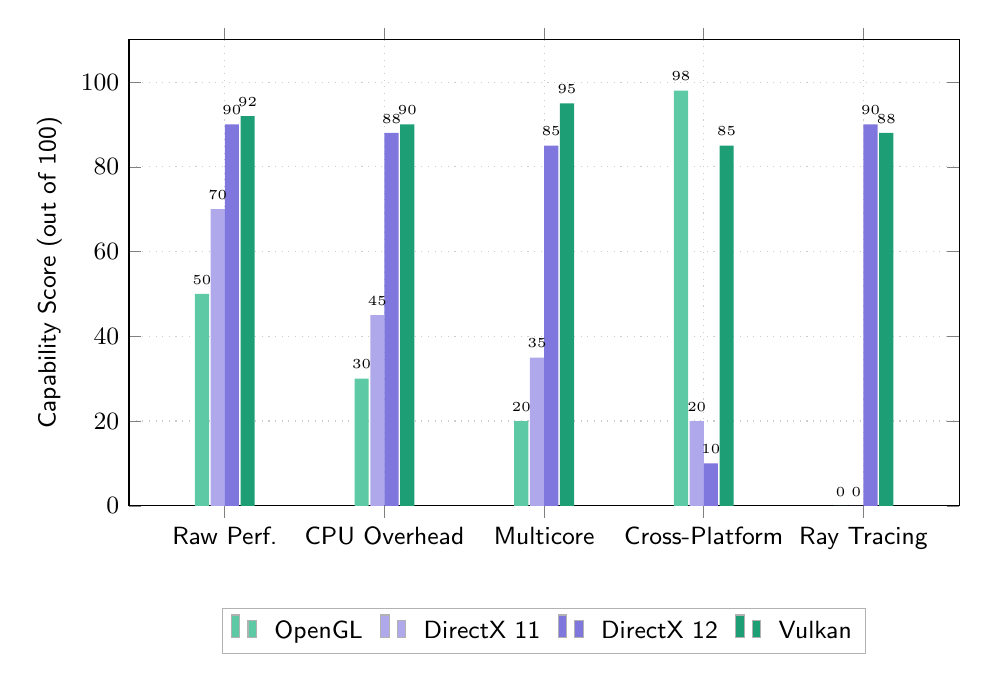
\begin{tikzpicture}
		\begin{axis}[
			ybar,
			bar width=0.18cm,
			width=\linewidth,
			height=7.5cm,
			enlarge x limits=0.15,
			ylabel={Capability Score (out of 100)},
			ylabel style={font=\small\sffamily},
			symbolic x coords={
				{Raw Perf.},
				{CPU Overhead},
				{Multicore},
				{Cross-Platform},
				{Ray Tracing}
			},
			xtick=data,
			xticklabel style={font=\small\sffamily},
			yticklabel style={font=\small\sffamily},
			ymin=0, ymax=110,
			ytick={0,20,40,60,80,100},
			grid=major,
			grid style={dotted, color=black!20},
			legend style={
				at={(0.5,-0.22)},
				anchor=north,
				legend columns=4,
				font=\small\sffamily,
				draw=black!30,
				column sep=1ex,
			},
			nodes near coords,
			nodes near coords style={
				font=\tiny\sffamily,
				/pgf/number format/fixed,
			},
			every axis plot/.append style={draw=none},
			]
			
			\addplot[fill={rgb,255:red,93;green,202;blue,165}, bar shift=-0.29cm]
			coordinates {
				({Raw Perf.},50)
				({CPU Overhead},30)
				({Multicore},20)
				({Cross-Platform},98)
				({Ray Tracing},0)
			};
			
			\addplot[fill={rgb,255:red,175;green,169;blue,236}, bar shift=-0.09cm]
			coordinates {
				({Raw Perf.},70)
				({CPU Overhead},45)
				({Multicore},35)
				({Cross-Platform},20)
				({Ray Tracing},0)
			};
			
			\addplot[fill={rgb,255:red,127;green,119;blue,221}, bar shift=0.09cm]
			coordinates {
				({Raw Perf.},90)
				({CPU Overhead},88)
				({Multicore},85)
				({Cross-Platform},10)
				({Ray Tracing},90)
			};
			
			\addplot[fill={rgb,255:red,29;green,158;blue,117}, bar shift=0.29cm]
			coordinates {
				({Raw Perf.},92)
				({CPU Overhead},90)
				({Multicore},95)
				({Cross-Platform},85)
				({Ray Tracing},88)
			};
			
			\legend{OpenGL, DirectX 11, DirectX 12, Vulkan}
		\end{axis}
	\end{tikzpicture}
	\caption*{\footnotesize\sffamily\color{gray}
		Graphics API capability comparison across five key dimensions. Scores are relative
		ratings derived from published benchmarks and API specifications, not a single-game benchmark.
		Sources: Basemark GPU, ARM Vulkan efficiency report, Android developer blog (Google, 2016),
		MoldStud Research (2025), GG Deals API comparison (2025).}
\end{figure}

\definecolor{nordBlue}{RGB}{94, 129, 172}
\definecolor{nordOrange}{RGB}{208, 135, 112}
\definecolor{moderngreen}{RGB}{163, 190, 140}
\definecolor{kernelGrey}{RGB}{128, 128, 128} 

\begin{figure}[H]
	\centering
	\begin{tikzpicture}[
		layer/.style={
			draw=#1!60, fill=#1!10, rounded corners=6pt,
			minimum width=9cm, minimum height=0.85cm,
			font=\small\sffamily\bfseries, text=#1!80,
			inner sep=8pt, align=center
		},
		sublabel/.style={
			font=\scriptsize\sffamily\color{black!50},
			align=center
		},
		arrow/.style={->, >=stealth, thick, black!40, shorten >=2pt, shorten <=2pt}
		]
		
		\node[layer=black] (game) at (0, 6)
		{Windows Game (.exe)};
		\node[sublabel] at (7, 6)
		{DirectX, Win32 API calls};
		
		\node[layer=nordBlue] (dxvk) at (0, 4.6)
		{DXVK / VKD3D-Proton};
		\node[sublabel] at (7, 4.6)
		{DirectX $\rightarrow$ Vulkan translation};
		
		\node[layer=nordOrange] (wine) at (0, 3.2)
		{Wine (Proton fork)};
		\node[sublabel] at (7, 3.2)
		{Windows API $\rightarrow$ Linux syscalls};
		
		\node[layer=moderngreen] (vulkan) at (0, 1.8)
		{Vulkan / Mesa / NVIDIA driver};
		\node[sublabel] at (7, 1.8)
		{Native Linux graphics stack};
		
		\node[layer=kernelGrey] (kernel) at (0, 0.4)
		{Linux Kernel};
		\node[sublabel] at (7, 0.4)
		{Hardware access};
		
		\draw[arrow] (game.south)   -- (dxvk.north);
		\draw[arrow] (dxvk.south)   -- (wine.north);
		\draw[arrow] (wine.south)   -- (vulkan.north);
		\draw[arrow] (vulkan.south) -- (kernel.north);
		
		\draw[thick, nordBlue!60, decorate,
		decoration={brace, amplitude=8pt, mirror}]
		(-4.8, 5.0) -- (-4.8, 2.9);
		\node[font=\footnotesize\sffamily\color{nordBlue!80}, align=center]
		at (-6.1, 3.95) {Proton\\layer};
		
	\end{tikzpicture}
	\caption*{\footnotesize\sffamily\color{gray}
		How Proton translates a Windows game into Linux-native calls. Based on
		\href{https://github.com/ValveSoftware/Proton}{ValveSoftware/Proton} and
		\href{https://github.com/doitsujin/dxvk}{DXVK} architecture documentation.}
\end{figure}

	
\begin{tcolorbox}[arc=12pt, outer arc=10pt,
	colback=blue!4!white, colframe=blue!40!black,
	title=\textbf{DXVK and VKD3D-Proton}]
	\textbf{DXVK} translates Direct3D 9, 10, and 11 calls into Vulkan.
	\textbf{VKD3D-Proton} (Valve's fork of VKD3D) translates Direct3D 12 calls into
	Vulkan. Together they handle the graphics API translation for virtually every
	modern Windows game. Vulkan is then handled natively by your GPU driver ---
	\code{nvidia} or \code{amdgpu}.
\end{tcolorbox}

\subsection{Setting Up Steam}

Launch Steam from the application launcher or by typing \code{steam} in the
terminal. Sign in with your Steam account. On first launch, Steam will download
and install runtime components, this may take several minutes.

\subsection{MangoHud and GameMode}

Two tools installed alongside Steam are worth configuring immediately: \textbf{MangoHud} is an overlay that displays real-time performance metrics (FPS, frametime, GPU usage, CPU usage, VRAM, and temperatures) in the corner
of the screen while gaming. Enable it for any game by adding the following to
its Steam launch options (right-click game $\rightarrow$ \menu{Properties}
$\rightarrow$ \menu{General} $\rightarrow$ \textbf{Launch Options}):

\begin{minted}{bash}
	MANGOHUD=1 %command%
\end{minted}

\noindent \textbf{GameMode} is a daemon developed by Feral Interactive that temporarily
applies system-level optimisations when a game launches, CPU governor changes,
GPU performance mode, and process priority adjustments. Enable it via launch
options:

\begin{minted}{bash}
	gamemoderun %command%
\end{minted}

Both can be combined:

\begin{minted}{bash}
	MANGOHUD=1 gamemoderun %command%
\end{minted}

\begin{tcolorbox}[arc=12pt, outer arc=10pt,
	colback=red!5!white, colframe=red!60!black,
	title=\textbf{Warning}]
	Always include \code{\%command\%} in Steam launch options. It represents the
	game executable itself. Omitting it means the game will not launch at all.
	Any prefix (\code{MANGOHUD=1}, \code{gamemoderun}) must come before
	\code{\%command\%}.
\end{tcolorbox}

\newpage
\section{Setting Up Steam and Proton}

With gaming packages installed, Steam is ready to launch. This section covers
logging in, enabling Proton, understanding game compatibility, and installing
Proton-GE for games that need extra help.

\subsection{Launching Steam and Enabling Proton}

Open Steam from the application launcher or run:

\begin{minted}{bash}
	steam
\end{minted}

Sign in with your Steam account. On first launch, Steam downloads runtime
components --- this takes a few minutes. Once ready:

\begin{enumerate}[leftmargin=1.5em, nosep, label={\arabic*.}]
	\item Open \menu{Steam, Settings}
	\item Navigate to \menu{Compatibility}
	\item Enable \textbf{Enable Steam Play for supported titles}
	\item Enable \textbf{Enable Steam Play for all other titles}
	\item Select the latest stable Proton version as the default compatibility tool
	\item Restart Steam when prompted
\end{enumerate}

\begin{callout}{\textbf{Enable Both Toggles}}
	The first toggle covers games Valve has tested and verified. The second covers
	everything else --- many of which run perfectly. Enable both and test games
	yourself rather than relying on Steam's conservative compatibility labels.
\end{callout}

\noindent Install any game from your library and click \textbf{Play}. Proton
handles the rest transparently --- no configuration needed for most titles.

\subsection{Checking Compatibility with ProtonDB}

Before installing a game, check its compatibility report on
\href{https://www.protondb.com}{protondb.com}. ProtonDB is a community database
of user-submitted reports detailing how well each game runs through Proton,
what tweaks were required, and which Proton version was used.

\begin{mdframed}[linewidth=1.5pt, linecolor=black!50, topline=true, bottomline=true,
	leftline=false, rightline=false, backgroundcolor=black!3]
	\small\itshape
	ProtonDB uses a medal system to rate game compatibility. Ratings are derived
	from community reports asking specific questions about what worked and what
	did not, rather than a single subjective score.\\[4pt]
	\normalfont\small ---
	\href{https://www.protondb.com}{ProtonDB}, as described in
	\href{https://boilingsteam.com/protondb-ratings-revised/}{Boiling Steam's
		ratings analysis}
\end{mdframed}

\subsubsection{Navigating and Interpreting Reports}

When evaluating a game on \href{https://protondb.com}{ProtonDB}, the tier badge 
is just the first data point. Because hardware configurations vary wildly, a 
"Gold" game might run flawlessly on AMD graphics but require custom launch 
arguments or environment variables on Nvidia proprietary setups.

To get an accurate assessment, filter user-submitted logs by your hardware profile, 
focusing on your GPU and distribution. Pay close attention to report age; older 
submissions often reference bugs that have since been patched in upstream Proton.

Furthermore, look for recurring configuration patterns in the comments. Users 
frequently share essential launch options, like \texttt{PROTON\_NO\_ESYNC=1}, 
which can instantly elevate a buggy "Bronze" experience to a stable, playable state. 
Checking these nuances ensures you do not prematurely pass on a title.



\newpage \noindent ProtonDB has six rating tiers: 

\vspace{1em}

% ProtonDB Medal Badges
\begin{figure}[H]
	\centering
	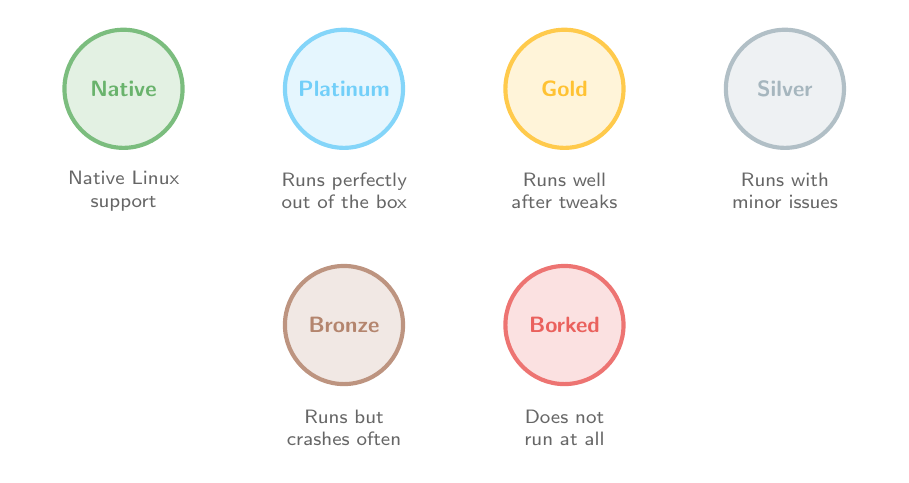
\begin{tikzpicture}[
		badge/.style={
			circle, draw=#1!70, fill=#1!15, line width=1.5pt,
			minimum size=1.5cm, font=\footnotesize\sffamily\bfseries,
			text=#1!80, align=center
		},
		desc/.style={
			font=\scriptsize\sffamily\color{black!60},
			text width=2.2cm, align=center
		}
		]
		
		\definecolor{platinumcol}{HTML}{4FC3F7}
		\definecolor{goldcol}{HTML}{FFB300}
		\definecolor{silvercol}{HTML}{90A4AE}
		\definecolor{bronzecol}{HTML}{A1664A}
		\definecolor{borkedcol}{HTML}{E53935}
		\definecolor{nativecol}{HTML}{43A047}
		
		\node[badge=nativecol]  (native)   at (0,    0) {Native};
		\node[badge=platinumcol](platinum) at (2.8,  0) {Platinum};
		\node[badge=goldcol]    (gold)     at (5.6,  0) {Gold};
		\node[badge=silvercol]  (silver)   at (8.4,  0) {Silver};
		\node[badge=bronzecol]  (bronze)   at (2.8, -3) {Bronze};
		\node[badge=borkedcol]  (borked)   at (5.6, -3) {Borked};
		
		\node[desc] at (0,    -1.3) {Native Linux\\support};
		\node[desc] at (2.8,  -1.3) {Runs perfectly\\out of the box};
		\node[desc] at (5.6,  -1.3) {Runs well\\after tweaks};
		\node[desc] at (8.4,  -1.3) {Runs with\\minor issues};
		\node[desc] at (2.8,  -4.3) {Runs but\\crashes often};
		\node[desc] at (5.6,  -4.3) {Does not\\run at all};
		
	\end{tikzpicture}
	\caption*{\footnotesize\sffamily\color{gray}
		ProtonDB rating tiers. Source:
		\href{https://www.protondb.com}{protondb.com} and
		\href{https://boilingsteam.com/protondb-ratings-revised/}{Boiling Steam}}
\end{figure}

\begin{callout}{\textbf{Ratings Are Not Final}}
	ProtonDB ratings are community-aggregated and most reports come from
	desktop Linux users running default Proton. A Silver rating might be Platinum
	on Proton-GE. A Bronze rating against an old Proton version might be Gold on
	the current release. Always check the recency of reports and try Proton-GE
	before giving up on a game. 
\end{callout}

\noindent Reports on ProtonDB often include the exact launch options, Proton
version, and system configuration used --- making them the most practical
source of per-game troubleshooting information available.

\subsection{Installing Proton-GE}

\textbf{Proton-GE} is an unofficial fork of Proton created and maintained by
a solo developer known as GloriousEggroll. It ships with additional components
not yet merged into Valve's official Proton:

\begin{itemize}[leftmargin=1.5em, nosep, label={\tiny\textbullet}]
	\item Media codec fixes for games with cutscene playback issues
	\item AMD FSR patches
	\item A per-game fix system that applies targeted workarounds automatically
	\item Patches from Wine and DXVK that Valve has not yet integrated
\end{itemize}

\noindent \code{protonup-qt} is already installed from the gaming packages
step. Open it from the application launcher:

\begin{enumerate}[leftmargin=1.5em, nosep, label={\arabic*.}]
	\item ProtonUp-Qt will automatically detect your Steam installation
	\item Click \textbf{Add version}
	\item Select \textbf{GE-Proton} as the compatibility tool
	\item Choose the latest GE-Proton version from the list
	\item Click \textbf{Install}: download and installation will begin
	\item Once complete, restart Steam
	\item Go to \menu{Steam, Settings, Compatibility} and select
	\textbf{GE-Proton} as the default, or set it per game
\end{enumerate}

\begin{tcolorbox}[arc=12pt, outer arc=10pt,
	colback=blue!4!white, colframe=blue!40!black,
	title=\textbf{Per-Game Proton Version}]
	You can set a specific Proton version for individual games without changing
	the global default. Right-click the game in your Steam library, select
	\menu{Properties}, navigate to \menu{Compatibility}, and check Force the use of a specific Steam Play compatibility tool. This
	is useful when one game runs best on official Proton while another needs
	Proton-GE.
\end{tcolorbox}

\begin{tcolorbox}[arc=12pt, outer arc=10pt,
	colback=red!5!white, colframe=red!60!black,
	title=\textbf{Warning}]
	Proton-GE is not officially supported by Valve. If a game breaks after
	switching to Proton-GE, switch back to the latest official Proton version
	first before reporting issues anywhere. Never report Proton-GE bugs to
	Valve's issue tracker --- report them to the
	\href{https://github.com/GloriousEggroll/proton-ge-custom}{GloriousEggroll
		GitHub repository} instead.
\end{tcolorbox}

\newpage
\section{Setting Up Lutris}

\begin{mdframed}[linewidth=1.5pt, linecolor=black!50, topline=true, bottomline=true,
	leftline=false, rightline=false, backgroundcolor=black!3]
	\small\itshape
	``Lutris is a free and open source game manager for Linux-based operating systems
	developed and maintained by Mathieu Comandon and the community, released under the
	GNU General Public License.''\\[4pt]
	\normalfont\small ---
	\href{https://en.wikipedia.org/wiki/Lutris}{Wikipedia: Lutris},
	citing \href{https://lutris.net}{lutris.net}
\end{mdframed}

\noindent Lutris is the tool that fills the gap Steam leaves. It manages games from
GOG, Epic Games, emulators, and any Windows game installed manually through Wine ---
all from a single interface. For games sourced outside of Steam, Lutris is the
primary solution on Linux.

\begin{callout}{\textbf{Run Lutris from the Terminal}}
	It is good practice to launch Lutris from the terminal rather than the application
	launcher:
	\begin{minted}{bash}
		lutris
	\end{minted}
	This prints Lutris logs and Wine/Proton output directly to the terminal in real
	time. When something goes wrong, this output is what you paste when asking for
	help online.
\end{callout}

\subsection{Key Concepts Before You Start}

\begin{tcolorbox}[arc=12pt, outer arc=10pt,
	colback=blue!4!white, colframe=blue!40!black,
	title=\textbf{What is a Runner?}]
	According to the \href{https://lutris.net/faq}{official Lutris FAQ}, a
	\textbf{runner} is any program capable of running games --- Wine, DOSBox, MAME,
	Linux itself, and others. For Windows games, the runner is \textbf{Wine} or a
	Proton-based Wine build. The runner is configured per game and determines how
	Lutris launches the executable.
\end{tcolorbox}

\begin{tcolorbox}[arc=12pt, outer arc=10pt,
	colback=blue!4!white, colframe=blue!40!black,
	title=\textbf{What is a Wine Prefix?}]
	A Wine prefix is an isolated directory that simulates a Windows environment ---
	a fake \directory{C:} drive, a Windows registry, and DLL files. Each game gets
	its own prefix by default in Lutris, stored under
	\directory{~/Games/}. This isolation means one game's Wine configuration cannot
	break another's. Lutris manages prefixes automatically --- you do not need to
	create or configure them manually. The Tweaks section covers manual prefix
	management in detail.
\end{tcolorbox}

\subsection{Configuring GE-Proton as the Default Runner}

Before adding any games, set GE-Proton as the default Wine version in Lutris:

\begin{enumerate}[leftmargin=1.5em, nosep, label={\arabic*.}]
	\item Open \menu{Lutris, Preferences}
	\item Navigate to \menu{Global options, Wine version}
	\item Select the latest \textbf{GE-Proton} build from the dropdown
\end{enumerate}

\noindent If GE-Proton does not appear in the list, open \textbf{ProtonUp-Qt},
select \textbf{Lutris} as the target, and install the latest GE-Proton version
from there. Restart Lutris after installation.

\subsection{Adding Games to Lutris}

There are two paths depending on what you have:

\vspace{1em}

\definecolor{nordBlue}{RGB}{94, 129, 172}
\definecolor{moderngreen}{RGB}{163, 190, 140}
\definecolor{moderngreenlight}{RGB}{236, 243, 230}

	
	% Decision Flowchart
	\begin{figure}[H]
		\centering
		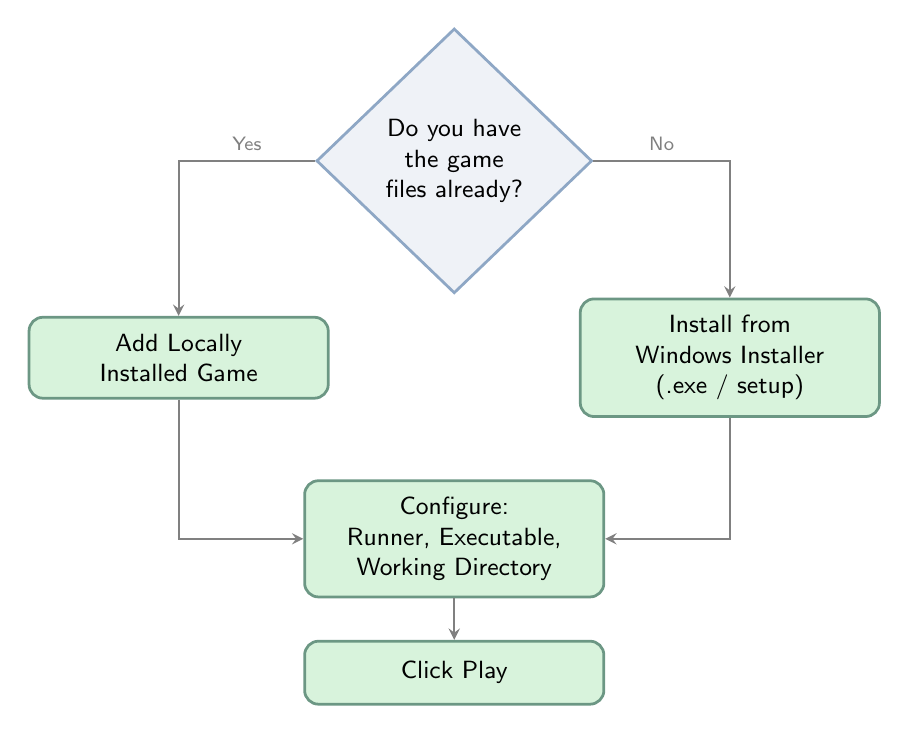
\begin{tikzpicture}[
			decision/.style={
				diamond, draw=nordBlue!70, fill=nordBlue!10, line width=1pt,
				font=\small\sffamily, inner sep=4pt, align=center,
				minimum width=3.5cm, minimum height=1.2cm
			},
			action/.style={
				rounded corners=5pt, draw=moderngreen!70, fill=moderngreenlight,
				line width=1pt, font=\small\sffamily, inner sep=6pt,
				align=center, minimum width=3.8cm, minimum height=0.8cm
			},
			arrow/.style={->, >=stealth, thick, black!50}
			]
			
			\node[decision] (q1) at (0, 0)
			{Do you have\\the game\\files already?};
			
			\node[action] (portable) at (-3.5, -2.5)
			{Add Locally\\Installed Game};
			
			\node[action] (installer) at (3.5, -2.5)
			{Install from\\Windows Installer\\(.exe / setup)};
			
			\node[action] (config) at (0, -4.8)
			{Configure:\\Runner, Executable,\\Working Directory};
			
			\node[action] (play) at (0, -6.5)
			{Click Play};
			
			\draw[arrow] (q1.west) -- node[above, font=\scriptsize\sffamily]{Yes}
			(-3.5, 0) -- (portable.north);
			\draw[arrow] (q1.east) -- node[above, font=\scriptsize\sffamily]{No}
			(3.5, 0) -- (installer.north);
			\draw[arrow] (portable.south) -- (-3.5, -4.8) -- (config.west);
			\draw[arrow] (installer.south) -- (3.5, -4.8) -- (config.east);
			\draw[arrow] (config.south) -- (play.north);
			
		\end{tikzpicture}
		\caption*{\footnotesize\sffamily\color{gray}
			Decision flow for adding a game to Lutris.
			Based on \href{https://lutris.net/faq}{Lutris FAQ} and
			\href{https://github.com/lutris/lutris}{Lutris GitHub documentation}.}
	\end{figure}
	
	

\subsection{Adding a Locally Installed or Portable Game}

Use this path if you already have the game files on disk, a portable install,
an extracted archive, or files copied from another system.

\subsubsection{Game Info Tab}

\begin{enumerate}[leftmargin=1.5em, nosep, label={\arabic*.}]
	\item Click the \textbf{+} icon in the top-left corner of the Lutris window
	\item Select \textbf{Add locally installed game}
	\item Enter the correct, full name of the game --- Lutris uses this to fetch
	metadata, cover art, and banner images from its database. An incorrect name
	produces no metadata
	\item Under \textbf{Runner}, select \textbf{Wine} --- this is the runner for
	all Windows games
\end{enumerate}

\subsubsection{Game Options Tab}

\begin{itemize}[leftmargin=1.5em, nosep, label={\tiny\textbullet}]
	\item \textbf{Executable} --- navigate to and select the game's \code{.exe} file
	\item \textbf{Arguments} --- leave blank unless the game requires specific
	launch arguments (documented on ProtonDB or the game's own documentation)
	\item \textbf{Working Directory} --- navigate to the directory containing the
	\code{.exe} file and select it. This is important: some games look for assets
	relative to their working directory and will fail if it is set incorrectly
	\item \textbf{Wine Prefix} --- leave empty. Lutris will create a fresh, isolated
	Wine prefix automatically for the game
\end{itemize}

\subsubsection{Runner Options Tab}

\begin{itemize}[leftmargin=1.5em, nosep, label={\tiny\textbullet}]
	\item \textbf{Wine version}: select the latest \textbf{GE-Proton} build
\end{itemize}

\noindent Click \textbf{Save}. The game will appear in your Lutris library.
Click \textbf{Play} to launch it.

\begin{callout}{\textbf{First Launch May Be Slow}}
	On first launch, Lutris downloads Wine dependencies and initialises the Wine
	prefix. This can take a minute or two. Subsequent launches are immediate.
	Monitor progress by right-clicking the game and selecting \textbf{Show logs}.
\end{callout}

\subsection{Installing a Game from a Windows Installer}

Use this path if you have a setup file, a GOG offline installer, a standalone
\code{setup.exe}, or a repacked installer.

\begin{enumerate}[leftmargin=1.5em, nosep, label={\arabic*.}]
	\item Click the \textbf{+} icon in the top-left corner
	\item Select \textbf{Install a Windows game from an executable}
	\item Enter the game name and click \textbf{Install}
	\item Choose an installation directory, creating a dedicated folder under
	\directory{~/Games/} is recommended, e.g.\ \directory{~/Games/GameName/}
	\item Navigate to and select the \code{setup.exe} or installer file
	\item Complete the installation wizard as you would on Windows
	\item Click \textbf{Close} when finished
\end{enumerate}

\noindent The game will appear in your Lutris library, but requires one more
configuration step. Right-click the game and select \textbf{Configure}:

\subsubsection{Game Info Tab}
\begin{itemize}[leftmargin=1.5em, nosep, label={\tiny\textbullet}]
	\item Confirm \textbf{Runner} is set to \textbf{Wine}
\end{itemize}

\subsubsection{Game Options Tab}
\begin{itemize}[leftmargin=1.5em, nosep, label={\tiny\textbullet}]
	\item \textbf{Executable}: navigate to the game's main \code{.exe} file
	inside the installation directory you chose
	\item \textbf{Working Directory}: set to the directory containing that
	\code{.exe} file
	\item \textbf{Wine Prefix}: leave at the default value
\end{itemize}

\subsubsection{Runner Options Tab}
\begin{itemize}[leftmargin=1.5em, nosep, label={\tiny\textbullet}]
	\item \textbf{Wine version}: select the latest \textbf{GE-Proton} build
\end{itemize}

\noindent Click \textbf{Save}, then click \textbf{Play}.

\begin{tcolorbox}[arc=12pt, outer arc=10pt,
	colback=red!5!white, colframe=red!60!black,
	title=\textbf{Warning}]
	If the game does not launch, right-click it and select \textbf{Show logs}.
	The log output is the first thing any Linux gaming forum or subreddit will ask
	for. Do not ask for help without attaching it. Refer to the Troubleshooting
	section of this guide for common Lutris failure patterns.
\end{tcolorbox}

\begin{callout}{\textbf{GOG, Repacks, and Portable Files}}
	Prefer GOG offline installers or portable game files over repacks when possible.
	GOG installers are clean, official builds with no modifications. Repacks are
	compressed community repackages --- they work, but introduce an additional layer
	of complexity and are more prone to installation errors. A failed repack
	installation is harder to diagnose than a failed GOG installation.
\end{callout}

\end{document}



